%!TEX program = xelatex
\documentclass[dvipsnames, svgnames,a4paper,11pt]{article}
% ----------------------------------------------------- 
%	加边框的命令
%	参考:https://tex.stackexchange.com/questions/531559/how-to-add-the-page-border-for-first-two-pages-in-latex
\usepackage{tikz}
\usetikzlibrary{calc}
\usepackage{eso-pic}
\AddToShipoutPictureBG{%
\begin{tikzpicture}[overlay,remember picture]
\draw[line width=0.6pt] % 边框粗细
    ($ (current page.north west) + (0.6cm,-0.6cm) $)
    rectangle
    ($ (current page.south east) + (-0.6cm,0.6cm) $); % 边框位置
\end{tikzpicture}}


\usepackage{xcolor}
\definecolor{c1}{HTML}{070F94} % 目录颜色 原版为2752C9 紫灰色535AAA 蓝紫色0B0DB7 深蓝色070F94 湖绿色219394 松石灰绿086173
\definecolor{c2}{HTML}{E20129} % 引用颜色 原版\definecolor{c2}{RGB}{190,20,83} 橙色F24729

\usepackage{ctex}
\usepackage[top=28mm,bottom=28mm,left=15mm,right=15mm]{geometry}
\usepackage{hyperref} 
\hypersetup{
	colorlinks,
	linktoc = section, % 超链接位置,选项有section, page, all
	linkcolor = c1, % linkcolor 目录颜色
	citecolor = c1  % citecolor 引用颜色
}
\usepackage{amsmath,enumerate,multirow,float}
\usepackage{tabularx}
\usepackage{tabu}
\usepackage{subfig}
\usepackage{fancyhdr}
\usepackage{graphicx}
\usepackage{wrapfig}  
\usepackage{physics}
\usepackage{appendix}
\usepackage{amsfonts}

%
\usepackage{tcolorbox}
\tcbuselibrary{skins,breakable}
\newtcolorbox{tbox}[2][]{
    colframe=black!70!,
    breakable,
    enhanced,
	boxrule =0.5pt,
    title = {#2},
    fonttitle = \large\kaishu\bfseries,
	drop fuzzy shadow,
    #1
}
\newtcolorbox[auto counter,number within=section]{question}[1][]{
  top=2pt,bottom=2pt,arc=1mm,
  boxrule=0.5pt,
%   frame hidden,
  breakable,
  enhanced, %跨页后不会显示下边框
  coltitle=c1!80!gray,
  colframe=c1,
  colback=c1!3!white,
  drop fuzzy shadow,
  title={思考题~\thetcbcounter:\quad},
  fonttitle=\bfseries,
  attach title to upper,
  #1
}

% ---------------------------------------------------------------------
%	利用cleveref改变引用格式,\cref是引用命令
\usepackage{cleveref}
\crefformat{figure}{#2{\textcolor{c2}{Figure #1}}#3} % 图片的引用格式
\crefformat{equation}{#2{(\textcolor{c2}{#1})}#3} % 公式的引用格式
\crefformat{table}{#2{\textcolor{c2}{Table #1}}#3} % 表格的引用格式


% ---------------------------------------------------------------------
%	页眉页脚设置
\fancypagestyle{plain}{\pagestyle{fancy}}
\pagestyle{fancy}
\lhead{\kaishu 中山大学物理与天文学院基础物理实验\uppercase\expandafter{\romannumeral2}} % 左边页眉,学院 + 课程
\rhead{\kaishu 实验报告By黄罗琳} % 右边页眉,实验报告标题
\cfoot{\thepage} % 页脚,中间添加页码


% ---------------------------------------------------------------------
%	对目录、章节标题的设置
\renewcommand{\contentsname}{\centerline{\huge 目录}}
\usepackage{titlesec}
\usepackage{titletoc}
% \titleformat{章节}[形状]{格式}{标题序号}{序号与标题间距}{标题前命令}[标题后命令]
\titleformat{\section}{\centering\LARGE\songti}{}{1em}{}

% ---------------------------------------------------------------------
%   listing代码环境设置
\usepackage{listings}
\lstloadlanguages{python}
\lstdefinestyle{pythonstyle}{
backgroundcolor=\color{gray!5},
language=python,
frameround=tftt,
frame=shadowbox, 
keepspaces=true,
breaklines,
columns=spaceflexible,                   
basicstyle=\ttfamily\small, % 基本文本设置,字体为teletype,大小为scriptsize
keywordstyle=[1]\color{c1}\bfseries, 
keywordstyle=[2]\color{Red!70!black},   
stringstyle=\color{Purple},       
showstringspaces=false,
commentstyle=\ttfamily\scriptsize\color{green!40!black},%注释文本设置,字体为sf,大小为smaller
tabsize=2,
morekeywords={as},
morekeywords=[2]{np, plt, sp},
numbers=left, % 代码行数
numberstyle=\it\tiny\color{gray}, % 代码行数的数字字体设置
stepnumber=1,
rulesepcolor=\color{gray!30!white}
}




% ---------------------------------------------------------------------
%	其他设置
\def\degree{${}^{\circ}$} % 角度
\graphicspath{{./images/}} % 插入图片的相对路径
\allowdisplaybreaks[4]  %允许公式跨页 
\usepackage{lipsum}
\usepackage{adjustbox}
\usepackage{amsmath, amssymb}
\usepackage{booktabs} % 为表格提供更美观的线条
\usepackage{longtable} % 允许表格跨页
\usepackage{booktabs} % 用于 \toprule 和 \bottomrule
\usepackage{float} % 用于控制浮动行为
\usepackage{geometry} % 可用于调整表格的布局

%\usepackage{mathrsfs} % 字体
%\captionsetup[figure]{name=Figure} % 图片形式
%\captionsetup[table]{name=Table} % 表格形式
\begin{document}
	
	% 实验报告封面	
	% 顶栏
	\begin{table}
		\renewcommand\arraystretch{1.7}
		\begin{tabularx}{\textwidth}{
				|X|X|X|X
				|X|X|X|X|}
			\hline
			\multicolumn{2}{|c|}{预习报告}&\multicolumn{2}{|c|}{实验记录}&\multicolumn{2}{|c|}{分析讨论}&\multicolumn{2}{|c|}{总成绩}\\
			\hline
			\LARGE25 & & \LARGE25 & & \LARGE30 & & \LARGE80 & \\
			\hline
		\end{tabularx}
	\end{table}
	% ---
	
	% 信息栏
	\begin{table}
		\renewcommand\arraystretch{1.7}
		\begin{tabularx}{\textwidth}{|X|X|X|X|}
			\hline
			年级、专业: & 2022级 物理学 &组号: &实验组1 \\
			\hline
			姓名: &  黄罗琳  & 学号: & 22344001  \\
			\hline
			实验时间: & 2024/4/25 & 教师签名: & \\
			\hline
		\end{tabularx}
	\end{table}
	% ---
	
	% 大标题
	\begin{center}
		\LARGE CA2 \quad 夫兰克-赫兹实验:原子定态能级的观测
	\end{center}
	% ---
	
	% 注意事项
	
	% 基本
	\textbf{【实验报告注意事项】}
	\begin{enumerate}
		\item 实验报告由三部分组成:
		\begin{enumerate}
			\item 预习报告:课前认真研读实验讲义,弄清实验原理;实验所需的仪器设备、用具及其使用、完成课前预习思考题;了解实验需要测量的物理量,并根据要求提前准备实验记录表格(可以参考实验报告模板,可以打印)。\textcolor{red}{\textbf{(20分)}}
			\item 实验记录:认真、客观记录实验条件、实验过程中的现象以及数据。实验记录请用珠笔或者钢笔书写并签名(\textcolor{red}{\textbf{用铅笔记录的被认为无效}})。\textcolor{red}{\textbf{保持原始记录,包括写错删除部分,如因误记需要修改记录,必须按规范修改。}}(不得输入电脑打印,但可扫描手记后打印扫描件);离开前请实验教师检查记录并签名。\textcolor{red}{\textbf{(30分)}}
			\item 数据处理及分析讨论:处理实验原始数据(学习仪器使用类型的实验除外),对数据的可靠性和合理性进行分析;按规范呈现数据和结果(图、表),包括数据、图表按顺序编号及其引用;分析物理现象(含回答实验思考题,写出问题思考过程,必要时按规范引用数据);最后得出结论。\textcolor{red}{\textbf{(30分)}}
		\end{enumerate}
		\textbf{实验报告就是将预习报告、实验记录、和数据处理与分析合起来,加上本页封面。\textcolor{red}{(80分)}}
		\item 每次完成实验后的一周内交\textbf{实验报告}(特殊情况不能超过两周)。
	
		
	\end{enumerate}
	
	% 安全
	\textbf{【实验安全注意事项】}	
	\begin{enumerate}
		\item 连线时务必注意,接错线路容易毁坏 F-H 管。
		\item 连线时,$ V_{G2K}$加速电压端接高压, 使用过程中请勿触碰接线端
	\end{enumerate}
	
	% 目录
	\clearpage
	\tableofcontents
	\clearpage
	% ---
	
	
	
	% 预习报告	
	
	% 小标题
	\setcounter{section}{0}
	\section{CA2 夫兰克-赫兹实验:原子定态能级的观测\quad\heiti 预习报告}
	% ---
	
	% 实验目的
	\subsection{实验目的}
	\begin{enumerate}
		\item 从实验了解原子定态能级(量子化),更好掌握量子力学的基础知识。
		\item 训练建立微观物理过程与宏观物理量之间关系的能力。
		\item (选)学习分解多因素,研究独立因素影响实验现象的规律。
	\end{enumerate}
	% ---
	
	% 仪器用具
	\subsection{仪器用具}
	\begin{figure}[{H}]
		\centering
		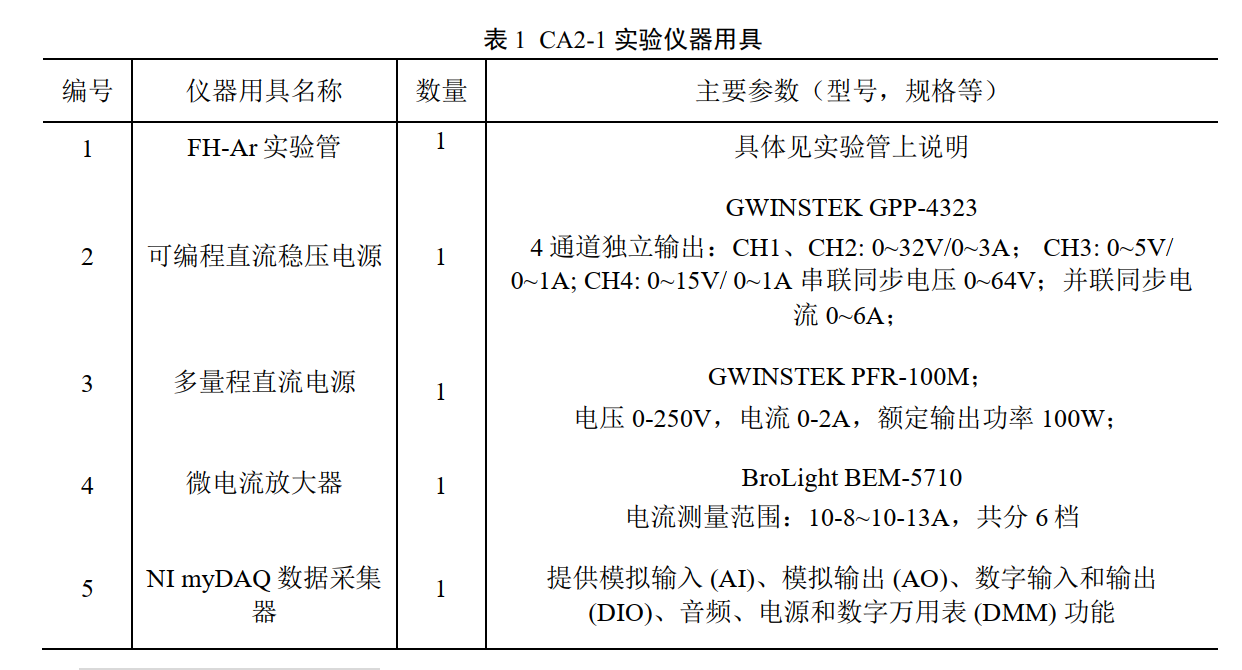
\includegraphics[width=0.9\linewidth]{仪器.png}
		\label{}
	\end{figure}
	% ---
	
	% 原理概述
	\subsection{原理概述}
	弗兰克-赫兹实验通过观察电子与原子碰撞时能量的转移来研究原子的能级结构。在该实验中,原子可以通过吸收或释放特定量的能量来在不同能级之间跃迁。这种能量的改变与辐射频率 $\nu$ 相关,关系式为:

$$
h\nu = E_n - E_m
$$

其中,$h$ 是普朗克常数,$E_n$ 和 $E_m$ 分别是原子的两个不同能级。


$$
e\Delta V=E_n-E_m
$$

\textbf{原子发生碰撞的电子能量达到$(E_n-E_m)$,原子未必会发生能级跃迁。
电子与原子碰撞后,能量未必完全传递给原子,若传递的能量小于$(E_n-E_m)$, 原子无法发生能级跃迁。
}


弗兰克-赫兹实验利用一个装有氩气的三极管,称为弗兰克-赫兹管(F-H 管),来进行实验。该管由一个热阴极(K),一个栅极(G),和一个阳极(P)组成。电子从热阴极发射,并在阴极和栅极之间的电场中被加速,电压记作 $V_{G_\mathrm{z}K}$. 当电子在加速过程中与氩原子碰撞时,电子的动能可能转移给氩原子,导致氩原子从一个能级跃迁到另一个能级。同时,电子的动能降低。在这种情况下,阳极与栅极之间的反向推斥电压 $V_{G_2P}$ 将会将能量不足的电子拉回。

图 1 显示了 F-H 管的实验原理图,其中展示了电子加速和与氩原子碰撞的过程。

$V_{G_{2k}}-V_{G_{1k}min}\leqslant V_{G_{2p}}$,电子不能抵达板极( 即图2a 点);
随着$V_{G_{2k}}$逐渐加大,当$V_{G_{2k}}$-$V_{G_{1k-min}}\gg V_{G_{2p}}$时,板极电流$I_{P}$将随$V_{G_{2k}}$ 的增加而增大(ab 段);

当$(V_{G_{2k}}-V_{G_{1k}min})$$\times e$>$E_n$-$E_m$时,电子与氩原子发生非弹性碰撞, 电子损失能量$(E_n-E_m)$, 电子即使穿过了G2 也不能克服反向拒斥电场而被折回第二栅极,则板极电流$I_P$将显著减小( bc 段);

随着$V_{G_{2k}}$进一步增加,电子继续加速,能量再次随之增加,使之可以克服反向拒斥电场而达到板极P,这时$I_{\mathcal{P}}$又再次上升( cd 段), 直到$V_{G_{2k}}$二倍于氩原子的第一激发电位以上时,电子因二次碰撞而又失去能量,造成第二次$I_{P}$的下降( de 段)。





\begin{figure}[H]
	\centering
	% 使用 minipage 设置并排的布局
	\begin{minipage}{0.25\textwidth} % 左边图片占总宽度的45%
		\centering
		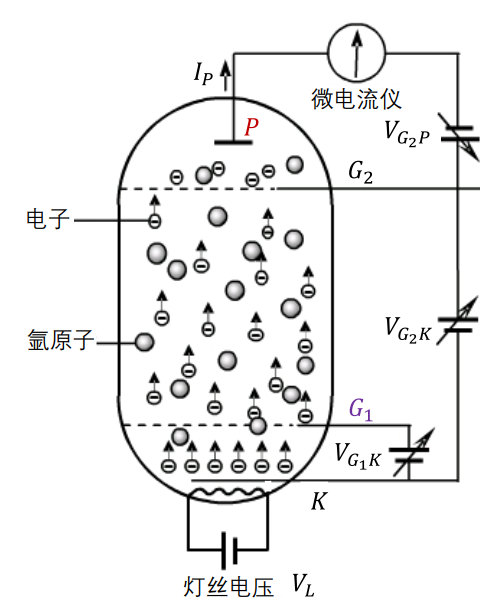
\includegraphics[width=\linewidth]{原理图.png} % 替换为你的图片路径
		\caption{实验原理图}
	\end{minipage}
	\begin{minipage}{0.55\textwidth} % 右边图片占总宽度的45%
		\centering
		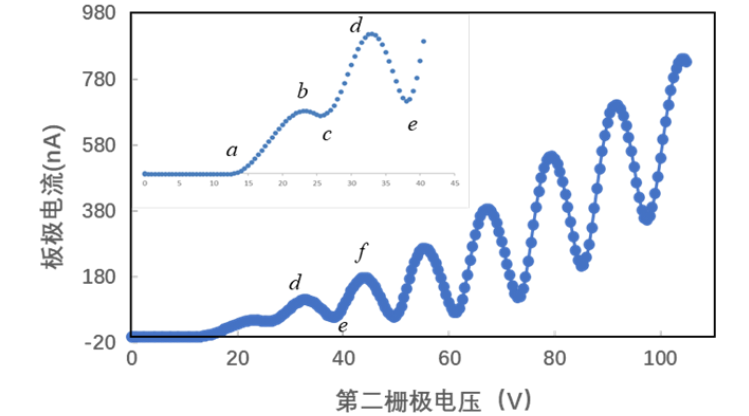
\includegraphics[width=\linewidth]{原理图3.png} % 替换为你的图片路径
		\caption{$I_P{\sim}V_{G_2K}$ 曲线}
	\end{minipage}
\end{figure}

\textbf{实验的预期现象:}当电子在 KG 区域加速到一定动能后,它们可能会在 GP 区域与氩原子碰撞,导致部分能量损失。如果这些电子的动能小于反向推斥电压 $V_{G_2P}$,它们将不会到达阳极,从而导致阳极电流减少。这一现象导致了阳极电流的周期性变化,表现为$I_{P}$随加速电压 $V_{G_2K}$ 变化的峰值和谷值。



\textbf{实验测量得到的结果为散点值,}为了精确得到$I_{P}-V_{G_{2}K}$曲线的峰值和谷值, 可以利用Python代码对实验数据进行拟合,进而找到曲线的峰值和谷值。


\textbf{如果 F-H 管内没有氩气,}电子将不会与原子碰撞并失去能量,因此阳极电流会随 $V_{G_2K}$ 单调增加,不会出现周期性的变化。


\textbf{对于从阴极发射出来的,但又不能抵达板极的那些电子}:当从阴极发射的电子无法抵达板极时,它们最终的去向可能有多种途径。首先,这些电子可能会在运动过程中与气体分子或其他物质发生碰撞,导致它们散射或被吸收。其次,这些电子可能会在极板之间的空间中反复运动,最终返回到阴极或其他电极上。此外,有些电子可能会由于具有足够的能量而逃逸出电场舒服,进入到器壁上。

\textbf{对于为什么不测G2板电流},是因为阳极电流是直接反映电子与气体原子碰撞的指标。阳极电流的下降表明电子与气体原子发生了非弹性碰撞,导致能量损失。测量阳极电流可以直接观察到气体原子的激发,验证量子力学中能级的概念。G2 极电流无法直接反映这些信息,无法准确预测有多少电子最终抵达阳极。

\textbf{并且测量G2板可能会使得实验所得数据并不明显,其主要是由于G2上拒斥电压的引入可以使一部分发生碰撞能量减少的电子并不能到达阳极,从而使得$I_P$减小,而若直接测量G2电流可能会使一些低能量的电子也可以进入到G2板上,出现较大本底电流,这样的最直接的结果就是实验结果不明显,甚至可能会出现反常结果的出现!}

\textbf{对于电子与氩原子发生弹性碰撞和非弹性碰撞的讨论}。

在这个过程中,电子的速度减小,而氩原子的速度增加。

理想状态下,电子在碰撞前的速度由加速电压 \(V\) 决定,计算公式为:
\[
v = \sqrt{ \frac{2eV}{m_e} }
\]

其中 \(e\) 是电子的电荷,\(m_e\) 是电子的质量。非弹性碰撞后,电子损失部分能量 \(\Delta E\),导致速度降低。碰撞后的电子速度变为:
\[
v' = \sqrt{ \frac{2(E - \Delta E)}{m_e} } = \sqrt{ \frac{2e(V - \Delta E)}{m_e} }.
\]

这种速度变化使电子的速度分布峰值向低速端移动,并可能导致分布的宽度增加,因为一部分电子减速,而另一部分可能保持原始速度。


对于氩原子来说,碰撞后获得部分电子的能量 \(\Delta E\),这使氩原子的动能增加。氩原子的速度可以通过以下公式计算:
\[
v_{\text{Ar}} = \sqrt{ \frac{2 \Delta E}{m_{\text{Ar}}} },
\]

\textbf{其中 \(m_{\text{Ar}} \approx 40 \, \text{amu}\) 是氩原子的质量。}

氩原子的速度分布取决于其激发或离子化所需的能量,不同的能量转移会导致不同的速度变化,但是总体上能量增加,并且可能出现二次碰撞。


此外对于电子在弹性碰撞下能量损失,设电子初始速度为 \(v_1\),碰撞后速度为 \(v_2\),而氩原子初始时是静止的。

根据动量守恒和能量守恒
\[
m_e \cdot v_1 = m_e \cdot v_2 + m_{\text{Ar}} \cdot v_{\text{Ar}}.
\]


\[
\frac{1}{2} m_e \cdot v_1^2 = \frac{1}{2} m_e \cdot v_2^2 + \frac{1}{2} m_{\text{Ar}} \cdot \left( \frac{m_e \cdot (v_1 - v_2)}{m_{\text{Ar}}} \right)^2.
\]

\[
\Delta E = \frac{1}{2} m_e \cdot v_1^2 - \frac{1}{2} m_e \cdot v_2^2.
\]

\[
\frac{\Delta E}{\frac{1}{2} m_e \cdot v_1^2}.
\]

当 \(m_{\text{Ar}} \gg m_e\) 时,氩原子的质量比电子大很多,电子速度的改变较小,电子的动能损失相对值也会非常小。这表明,弹性碰撞后电子损失的能量与其碰撞前动能相比可以忽略不计。








	% ---
	
	
	

	
	
	% 实验记录	
	\clearpage
	
	% 顶栏
	\begin{table}
		\renewcommand\arraystretch{1.7}
		\centering
		\begin{tabularx}{\textwidth}{|X|X|X|X|}
			\hline
			专业: & 物理学 & 年级: & 2022级 \\
			\hline
			姓名: & 黄罗琳 & 学号: & 22344001\\
			\hline
			室温: & 23℃ & 实验地点: & A509 \\
			\hline
			学生签名:& 
\includegraphics[width=1cm]{签字.jpg}& 评分: &\\
			\hline
			实验时间:& 2024/4/25 & 教师签名:&\\
			\hline
		\end{tabularx}
	\end{table}
	% ---
	
	% 小标题
	\section{CA2夫兰克-赫兹实验:原子定态能级的观测\quad\heiti 实验记录}
	% ---
	
	% 实验过程记录
	\subsection{实验内容、步骤与结果}
	
	%
	\subsubsection{操作步骤记录}
	\begin{enumerate}
	
  \item 控制参数及控制范围(工作点选取)

  F-H 管灯丝电流电压(CH4)、$V_{G_1K}$电压(CH1)、$V_{G_2P}$电压(CH2),根据FH-Ar 实验管上参数说明进行设置,过压电压值 OVP(V); 过流值 OCP(A)使用默认值。本次实验中设置$V_{G1k}=2V $\quad $V_{G2p}=8V$\quad $V_{L}=2V/1.8V/2.2V$
  实验起始电压和终止电压选用$0-85V$,步长选用1V。
  
  \textbf{对于工作点的选取}:按照装置参数表设置各电极电压,使得第一栅极$G_1$电压$V_{G_{1k}}$能够将电子从阴极周围拉出,使之持续发射电子又不至于过大将电子留在G1,使进入加速区的电子密度下降,默认参数基本为最佳工作环境,从而使得实验结果更加明显。

  \item 测量记录的物理量
  
  自动测量模式:$V_{G_2K}$电压将自动加压,计算机自动保存$V_{G_2K}$和$I_{P}$的数据。需要记录每次设置的$V_{L}$值,其余均使用默认参数。
  
  手动测量模式:$V_{L}=2V$直接通过电源面板设置$V_{G2K}$,在微电流放大器面板读电流值$I_{P}$,记录电流档位($10^{-9}$A)。

  \item 实验系统连接
  
  \begin{figure}[H]
	\begin{minipage}[b]{0.4\linewidth}
	  \centering
	  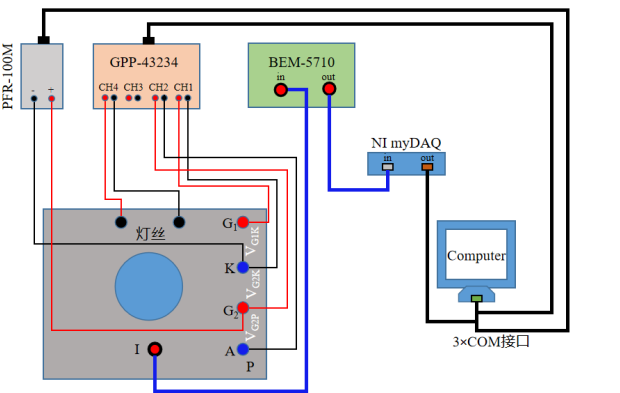
\includegraphics[width=0.9\linewidth]{接线.png}
	  \caption{实验系统接线}
	\end{minipage}
	\hfill
	\begin{minipage}[b]{0.4\linewidth}
	  \centering
	  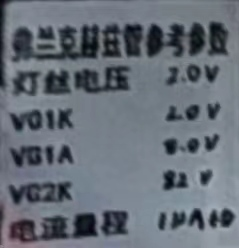
\includegraphics[width=0.5\linewidth]{参数.jpg}
	  \caption{仪器参数}
	\end{minipage}
  \end{figure}

  
  
  F-H 管灯丝电流电压(连 CH4)、$V_{G_1K}$电压(连 CH1)、$V_{G_2P}$电压(连 CH2), $G_2$ (连仪器PFR +极), $K$ (连仪器 PFR -极)。连线示意图如图4所示。
  \item 实验控制主界面操作
  
  Labview 程序主界面如下图所示,分为工作电压设置和自动测量两部分。相关参数设置和记录已在第1、2步中说明。
  \begin{figure}[H]
	\begin{minipage}[b]{0.4\linewidth}
	  \centering
	  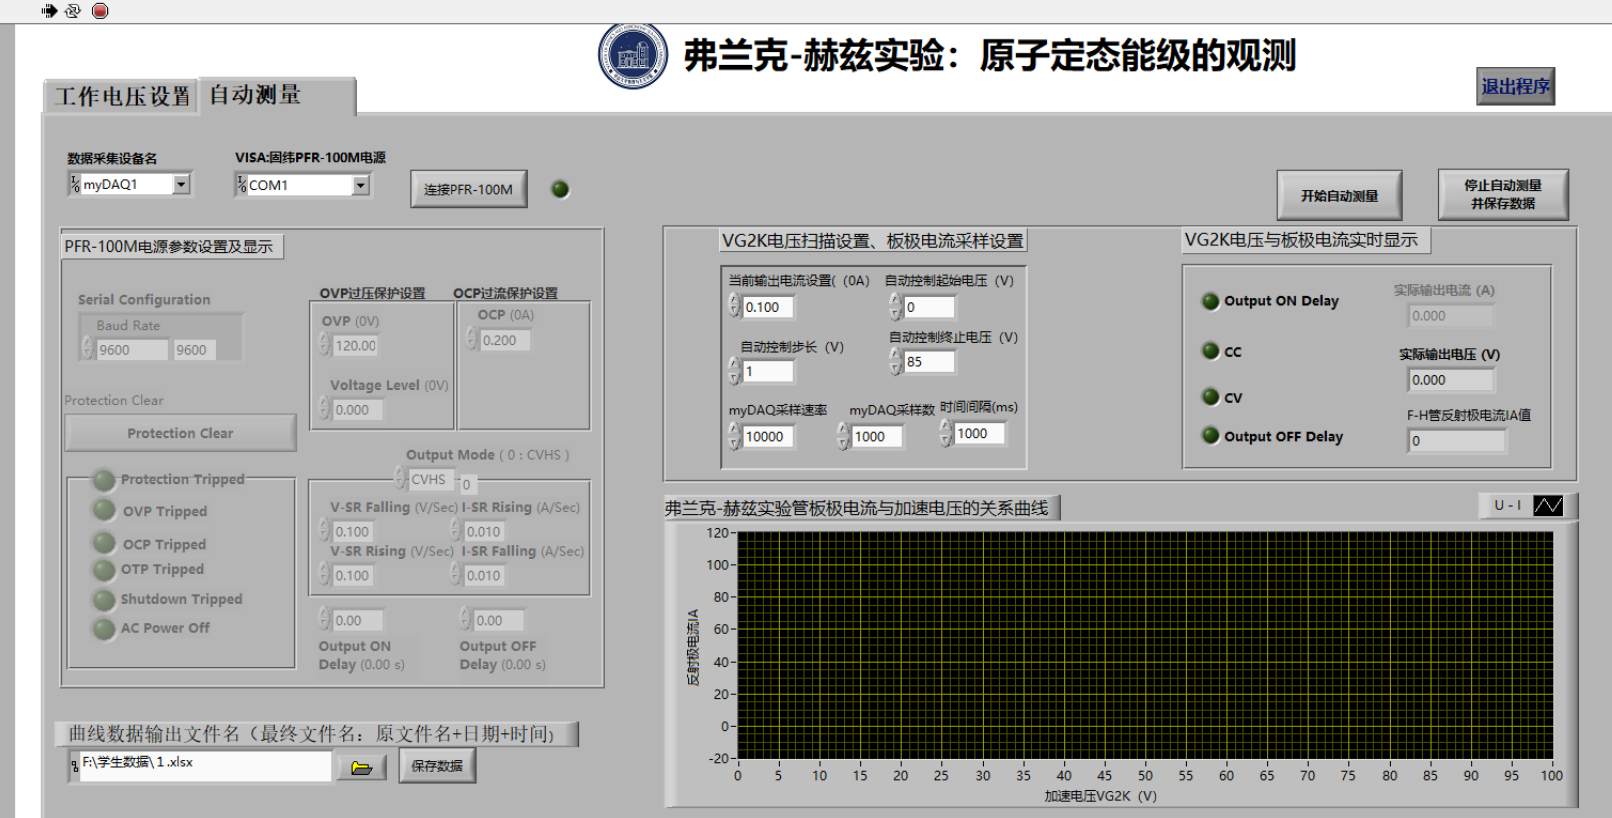
\includegraphics[width=\linewidth]{主界面.png}
	 
	\end{minipage}
	\hfill
	\begin{minipage}[b]{0.4\linewidth}
	  \centering
	  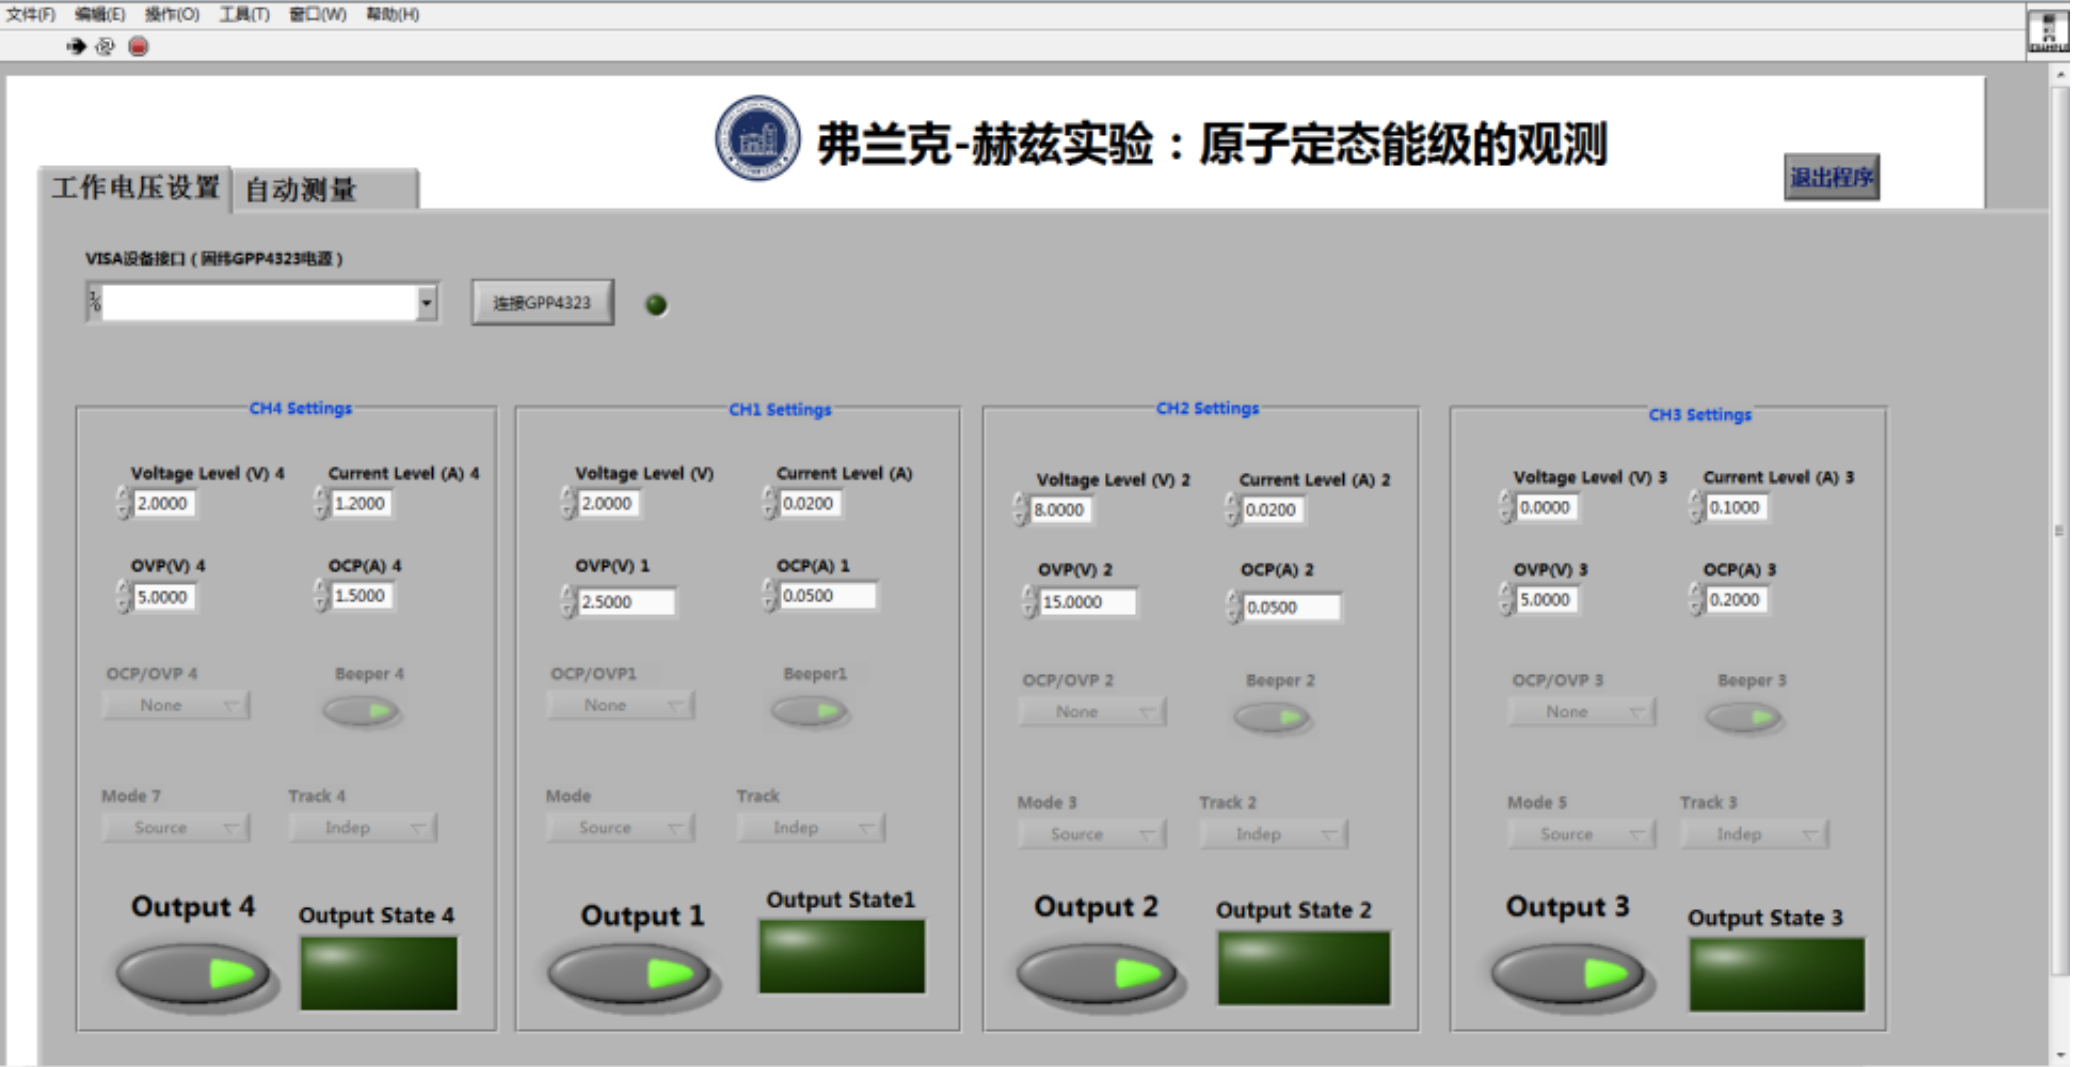
\includegraphics[width=\linewidth]{主界面2.png}
	  
	\end{minipage}
  \end{figure}
	\end{enumerate}	

	
	%
	\subsubsection{实验数据记录}
	
\begin{longtable}{|r|r|r|r|r|} % 5 列,第一列右对齐(r),其他四列居中
	\caption{电压与数据表} \\ % 表格标题
	\toprule

	
	
	
	$V_{G_2K}$ & 2V & 1.8V & 2.2V & 手动\\
	\midrule
	\endhead % 以下为表格内容
	0  & -9.694749  & -15.279422  & -16.892639  & 0   \\
	1  & -9.788475  & -15.216847  & -15.906743  & 0   \\
	2  & -9.874208  & -14.342165  & -14.630174  & 0   \\
	3  & -11.411665 & -12.292222  & -14.372565  & 0   \\
	4  & -5.867502  & -13.045717  & -13.547887  & 0   \\
	5  & -11.236373 & -12.144871  & -13.368155  & 0   \\
	6  & -11.310698 & -11.826463  & -8.49961   & 0   \\
	7  & -12.045748 & -11.574046  & -12.27125   & 0   \\
	8  & -11.964387 & -11.302159  & -11.924082  & 0   \\
	9  & -10.506037 & -10.586988  & -11.587572  & 2   \\
	10 & -11.474718 & -10.41074   & -5.400376  & 7   \\
	11 & -4.863639  & -5.976256   & 32.078027  & 19  \\
	12 & 4.368891   & 0.947629    & 103.907385 & 37  \\
	13 & 17.560035  & 10.109728   & 206.14958  & 52  \\
	14 & 32.922515  & 21.551781   & 295.373053 & 64  \\
	15 & 41.90577   & 23.399995   & 357.257033 & 71  \\
	16 & 48.125346  & 25.718682   & 390.375276 & 74  \\
	17 & 50.884722  & 25.330253   & 390.915771 & 69  \\
	18 & 49.672231  & 22.384587   & 350.413825 & 56  \\
	19 & 40.952391  & 15.84838    & 274.427881 & 44  \\
	20 & 27.906276  & 8.764505    & 184.330956 & 27  \\
	21 & 15.6556    & 2.082448    & 104.8318   & 15  \\
	22 & 5.742533   & -2.091011   & 51.72757   & 17  \\
	23 & 5.96947    & -2.436197   & 50.396624  & 32  \\
	24 & 14.509987  & 3.152916    & 122.034159 & 62  \\
	25 & 36.664029  & 13.64603    & 262.026643 & 91  \\
	26 & 65.679587  & 23.286937   & 402.970319 & 110 \\
	27 & 75.287088  & 30.19026    & 491.272452 & 115 \\
	28 & 84.308052  & 32.556424   & 517.358534 & 110 \\
	29 & 79.530568  & 30.233229   & 485.168872 & 92  \\
	30 & 70.607907  & 24.251246   & 397.075641 & 60  \\
	31 & 45.804405  & 15.292173   & 270.843555 & 39  \\
	32 & 24.288135  & 6.507914    & 146.312947 & 21  \\
	33 & 5.367904   & 0.97147     & 55.998785  & 11  \\
	34 & -0.120311  & -2.31337    & 15.822557  & 19  \\
	35 & 5.590605   & -0.329623   & 43.941435  & 46  \\
	36 & 24.192428  & 8.053023    & 158.864543 & 89  \\
	37 & 59.456048  & 19.957966   & 340.891374 & 127 \\
	38 & 90.594985  & 35.04808    & 505.402971 & 146 \\
	39 & 109.353519 & 37.556541   & 603.076583 & 154 \\
	40 & 115.445555 & 37.342106   & 626.839674 & 145 \\
	41 & 108.112132 & 35.251312   & 585.531838 & 123 \\
	42 & 90.187634  & 30.168673   & 488.153954 & 92  \\
	43 & 64.477001  & 21.93939    & 352.188739 & 59  \\
	44 & 39.94115   & 12.767454   & 210.774794 & 32  \\
	45 & 18.646147  & 5.93504     & 102.364873 & 21  \\
	46 & 7.251162   & 2.087503    & 47.005693  & 29  \\
	47 & 12.214185  & 4.616868    & 69.009719  & 62  \\
	48 & 35.465747  & 12.294521   & 188.907736 & 105 \\
	49 & 70.304937  & 23.433195   & 368.587188 & 145 \\
	50 & 104.196419 & 34.351149   & 539.933044 & 173 \\
	51 & 130.472616 & 41.766889   & 659.962085 & 187 \\
	52 & 140.185593 & 45.351693   & 714.675501 & 183 \\
	53 & 139.566129 & 44.867284   & 703.966722 & 165 \\
	54 & 124.804464 & 40.496947   & 634.550665 & 137 \\
	55 & 103.069934 & 33.594307   & 521.735771 & 104 \\
	56 & 75.823005  & 25.193012   & 384.953189 & 72  \\
	57 & 50.922226  & 17.210886   & 256.479678 & 50  \\
	58 & 34.052962  & 12.63356    & 167.86877   & 49  \\
	59 & 31.472703  & 14.264811   & 154.092318 & 71  \\
	60 & 47.785351  & 16.682006   & 225.759775 & 106 \\
	61 & 75.502616  & 24.709627   & 361.469908 & 148 \\
	62 & 108.100314 & 34.498705   & 520.588519 & 183 \\
	63 & 136.811604 & 43.449307   & 662.755822 & 207 \\
	64 & 157.665031  & 49.158788   & 762.403891 & 217 \\
	65 & 166.973867 & 52.006015   & 808.950326 & 214 \\
	66 & 164.108674 & 52.003829   & 797.980864 & 196 \\
	67 & 151.326795 & 47.364337   & 734.75897   & 170  \\
	68 & 134.94679  & 41.414461   & 632.146996  & 140 \\
	69 & 105.75191  & 34.668054   & 512.302059  & 115 \\
	70 & 85.022404  & 28.070979   & 405.136121  & 99  \\
	71 & 76.968481  & 25.001598   & 342.459093  & 103 \\
	72 & 76.513788   & 25.801409   & 347.31343   & 123 \\
	73 & 92.566368   & 30.233434   & 411.915866 & 153 \\
	74 & 112.799579   & 40.488817   & 524.373481 & 188  \\
	75 & 142.207118   & 45.131861   & 655.483198 & 218 \\
	76 & 169.027089   & 53.148348   & 778.624179  & 241 \\
	77 & 186.761061   & 58.089238   & 875.664528  & 256 \\
	78 & 199.612142   & 60.984078   & 932.753809   & 257 \\
	79 & 201.909037   & 60.365502   & 940.580863   & 248 \\
	80 & 194.41945   & 58.082338   & 904.641967   & 228 \\
	81 & 179.244559   & 53.944402   & 833.808   & 205 \\
	82 & 159.359062   & 50.180413   & 744.248426   & 185 \\
	83 & 142.561254   & 44.985534   & 665.73298   & 173 \\
	84 & 134.619023   & 42.162491   & 618.232415   & 175 \\
	85 & 136.027505   & 42.922271   & 616.382971   & 189 \\
	\bottomrule
	\end{longtable}
	% ---
	
	
	
	\subsection{实验过程遇到问题及解决办法}
	
		 实验中出现了接线错误的问题,为CH1和CH2的接线出现了对换,这就导致实验图像的显示并未出现峰谷交替,而是出现一个平缓的区域然后继续上升,之后通过助教老师的帮助下改正后完成了实验。

	% ---
	
	
	
	% 分析与讨论	
	\clearpage
	
	% 顶栏
	\begin{table}
		\renewcommand\arraystretch{1.7}
		\begin{tabularx}{\textwidth}{|X|X|X|X|}
			\hline
			专业:& 物理学 &年级:& 2022级\\
			\hline
			姓名: & 黄罗琳 & 学号:&22344001 \\
			\hline
			日期:&  2024/4/25& 评分: &\\
			\hline
		\end{tabularx}
	\end{table}
	% ---
	
	% 小标题
	\section{CA2 夫兰克-赫兹实验:原子定态能级的观测 \quad\heiti 分析与讨论}
	% ---
	
	% 数据处理
	\subsection{三组电压值实验数据分析}
	\subsubsection{实验数据绘图}
	
	对自动测量的三组数据,使用Python绘制拟合曲线,并标出峰谷点(代码见后)做出$I_P{\sim}V_{G_2K}$曲线
	\begin{figure}[{H}]
		\centering
		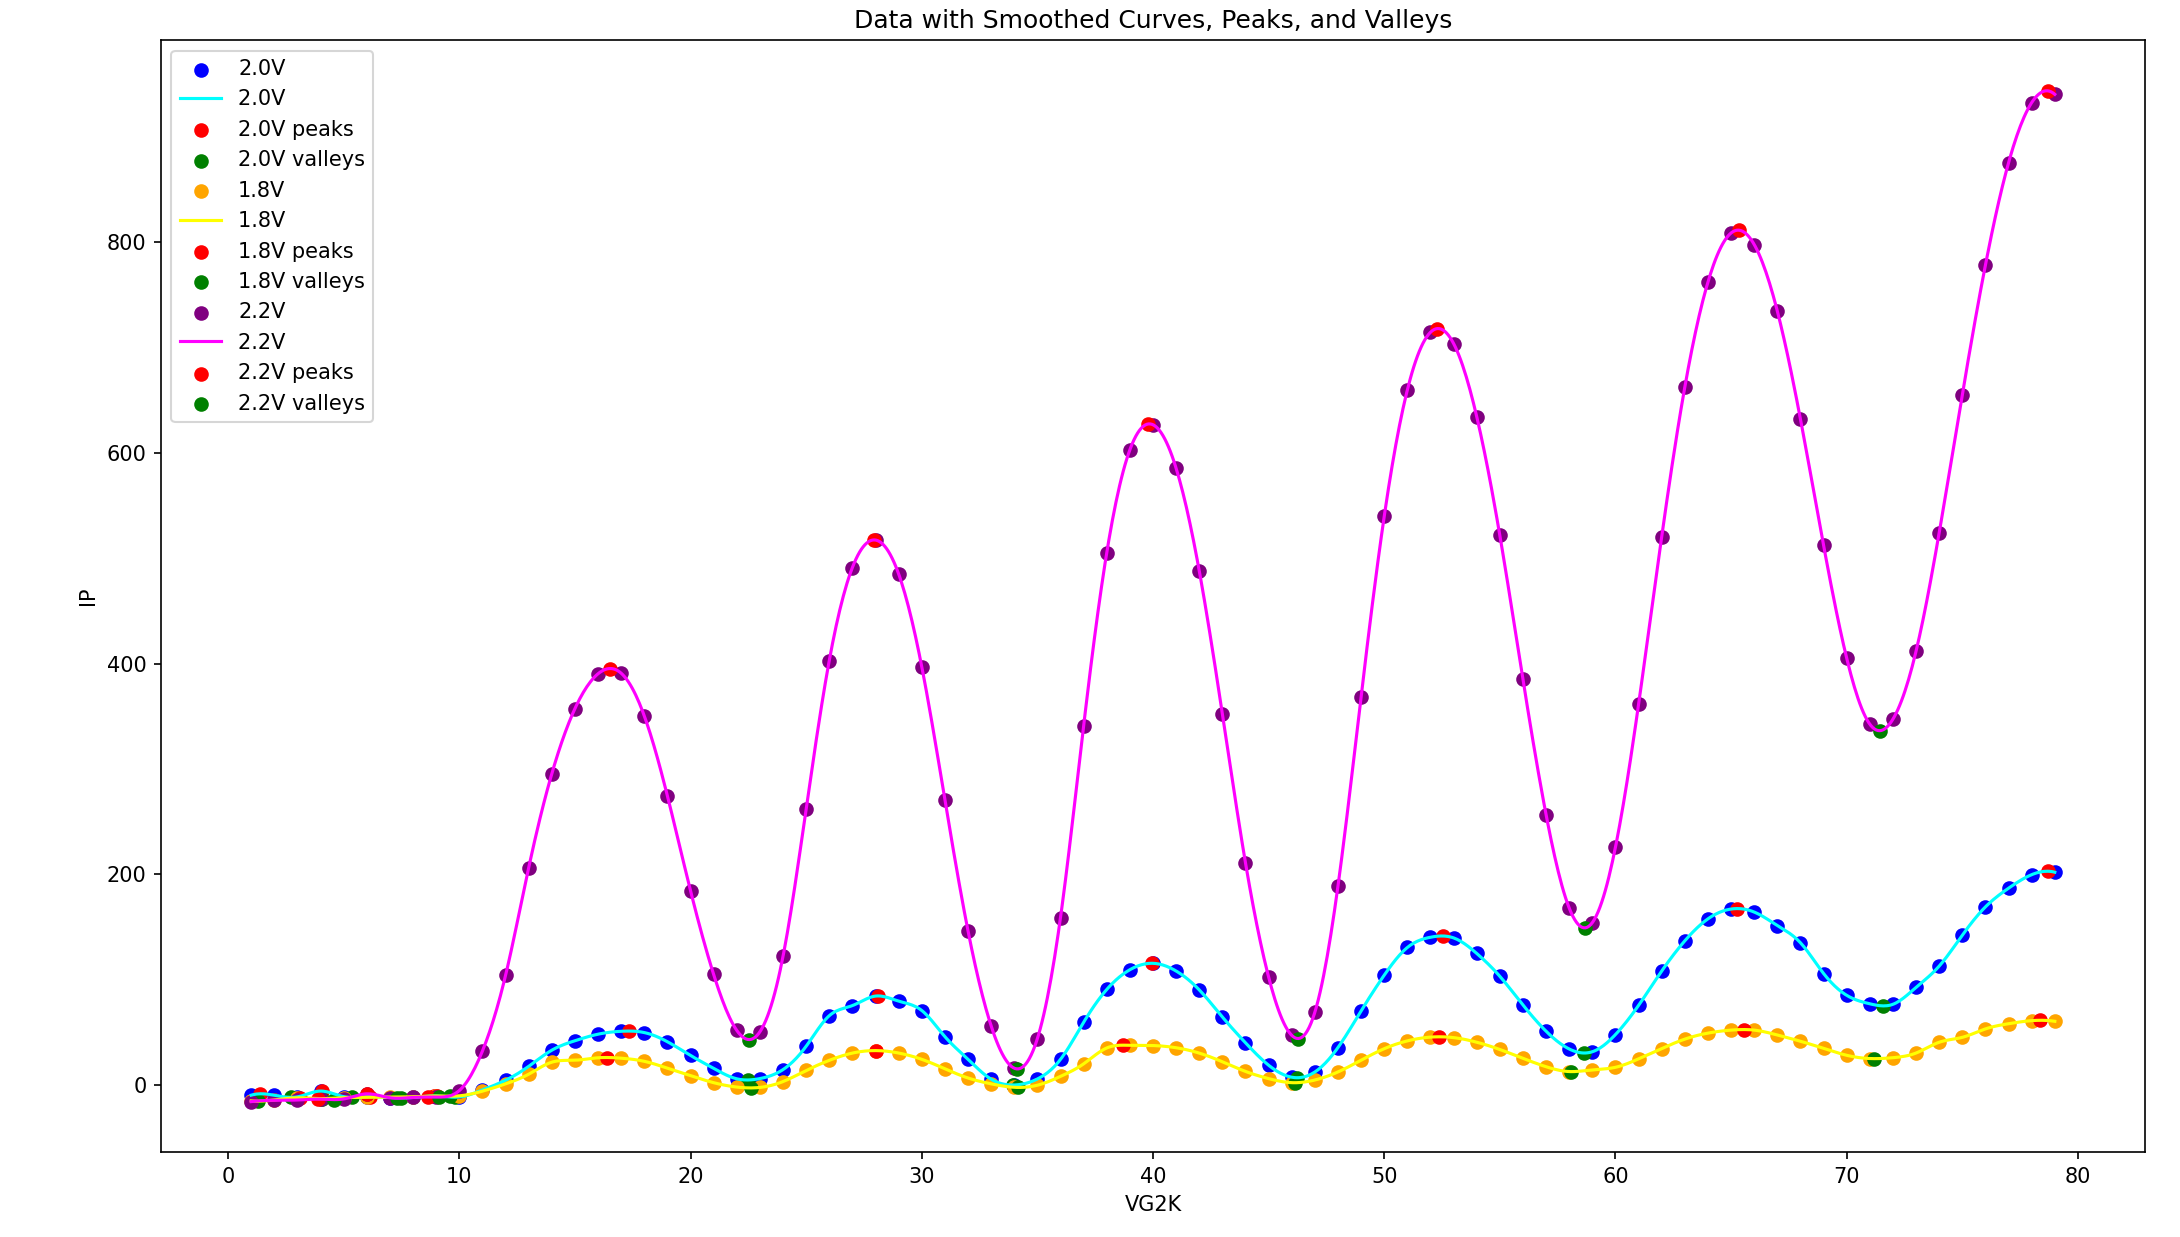
\includegraphics[width=0.65\linewidth]{拟合.png}
		\caption{曲线寻峰寻谷}
		\label{}
	\end{figure}
将此拟合图像中的相关数据提取出来,生成如下数据。
	\begin{table}[H]
		\centering\caption{拟合图像峰谷结果}
		\begin{tabular}{lcccccc}
		\hline
		 & 2.0V\_peaks & 2.0V\_valleys & 1.8V\_peaks & 1.8V\_valleys & 2.2V\_peaks & 2.2V\_valleys \\
		\hline
		0 & 1.390390 & 2.717718 & 3.108108 & 1.312312 & 3.888889 & 4.591592 \\
		1 & 4.045045 & 5.372372 & 9.042042 & 4.045045 & 5.996997 & 7.324324 \\
		2 & 6.153153 & 7.480480 & 16.381381 & 9.588589 & 8.651652 & 9.120120 \\
		3 & 8.885886 & 9.822823 & 28.015015 & 22.627628 & 16.537538 & 22.549550 \\
		4 & 17.318318 & 22.471471 & 38.711712 & 34.183183 & 27.936937 & 34.105105 \\
		5 & 28.093093 & 33.948949 & 52.375375 & 46.129129 & 39.804805 & 46.285285 \\
		6 & 39.960961 & 46.207207 & 65.570571 & 58.075075 & 52.297297 & 58.699700 \\
		7 & 52.531532 & 58.621622 & 78.375375 & 71.192192 & 65.336336 & 71.426426 \\
		\hline
		\end{tabular}
		
		\label{tab:example}
		\end{table}
		此实验数据存在较低电压时的拟合误差,故删除错误数据后,得出如下实验峰谷结果:
		\begin{table}[H]
			\centering\caption{拟合图像修正峰谷结果}
			\begin{tabular}{lcccccc}
			\hline
			 & 2.0V\_peaks & 2.0V\_valleys & 1.8V\_peaks & 1.8V\_valleys & 2.2V\_peaks & 2.2V\_valleys \\
			\hline
			1& 8.885886 & 9.822823 & 28.015015 & 22.627628 & 16.537538 & 22.549550 \\
			2 & 17.318318 & 22.471471 & 38.711712 & 34.183183 & 27.936937 & 34.105105 \\
			3 & 28.093093 & 33.948949 & 52.375375 & 46.129129 & 39.804805 & 46.285285 \\
			4 & 39.960961 & 46.207207 & 65.570571 & 58.075075 & 52.297297 & 58.699700 \\
			5 & 52.531532 & 58.621622 & 78.375375 & 71.192192 & 65.336336 & 71.426426 \\
			\hline
			\end{tabular}
			
			\label{tab:example}
			\end{table}
			计算每一组数据之间的峰-峰间距,谷-谷间距,得出如下结果,其中最后一行为各列数据取平均的结果。
			\begin{table}[H]
				\centering
				\caption{峰-峰、谷-谷间距}
				\label{tab:spacing_table}
				
				\begin{tabular}{rrrrrrrrrrrr}
				\toprule
				2.0V峰间距 & 2.0V谷间距 & 1.8V峰间距 & 1.8V谷间距  & 2.2V峰间距 & 2.2V谷间距  \\
				\midrule
			
				8.432432 & 12.648648 & 10.696697 & 11.555555 & 11.399399 & 11.555555 \\
				10.774775 & 11.477478 & 13.663663 & 11.945946 & 11.867868 & 12.180180 \\
				11.867868 & 12.258258 & 13.195196 & 11.945946 & 12.492492 & 12.414415 \\
				12.570571 & 12.414415 & 12.804804 & 13.117117 & 13.039039 & 12.726726 \\
				\hline
				10.911912 & 12.199200 & 12.590590 & 12.141641 & 12.199700 & 12.219719 \\
				\bottomrule
				\end{tabular}
				
				\end{table}
				所有数据的平均值为$\bar{V}_{0}=12.043794\mathrm{V}.$,$\text{其物理意义为氩原子的第一激发电位}$
\subsubsection{图像形状分析}
				分析图5所得实验图像,三组数据有着相似的实验图像,可以得出如实验原理概述中对于整体实验过程的描述:
				\begin{enumerate}
					\item 当$V_{G_{2k}}$逐渐加大时,刚开始$V_{G_{2k}}-V_{G_{1k}}\leqslant V_{G_{2p}}$, 电子不能抵达板极,故曲线在最初一段电流非常微弱几乎为零;
					\item 随着$V_{G_{2k}}$继续加大,当$V_{G_{2k}}-V_{G_{1k_{min}}}\geqslant V_{G_{2p}}$时,电子获得足够多的能量能够达到板极 P, 且$V_{G_{2k}}$越大,获得能量越多,故板极电流$I_{P}$将随$V_{G_{2k}}$的增加而增大;
					\item 当$(V_{G_{2k}}-V_{G_{1k_{min}}})$$\times e$>$E_{n}$-$E_{m}$时,电子与氩原子发生非弹性碰撞并损失能量($E_n$-$E_m$), 此时随着$V_{G_\mathrm{zk}}$继续加大板极电流$I_{P}$停止上升,形成第一个峰,之后由于电子不能到达极板,电流$I_{P}$不断减小,最终达到第一个谷.
					\item 随着$V_{G_{2k}}$进一步增加,电子继续加速,能量再次随之增加,使之可以克服反向拒斥电场而达到板极 P, 这时$I_\mathrm{p}$又再次上升,直到$V_{G_\mathrm{zk}}$二倍于氩原子的第一激发电位以上时,电子因二次碰撞而又失去能量。
					\item 第二次$I_{p}$的下降,以此类推。当$V_{G_{2k}}$的增量达到氩原子第一激发电位$V_0$整数倍时,微电流计检测出的电流都$I_{P}$都会开始下降,形成如图5所示起伏变化的$I_{P}{\sim}V_{G_{2k}}$曲线。
					
				\end{enumerate}
			\subsubsection{图像高度分析}
				观察图像可知,三组图像在有着相同峰谷位置的同时,电压$V_{G_2K}$相同,灯丝电压$V_{L}$越大,电流$I_P$越大,更高的电压会有更多的电子进入到容器中,从而使得电流更大。

					

	\subsection{两组不同方式实验数据分析}
	\subsubsection{实验数据绘图}
	对自动测量和手动测量($V_L=2.0V$)两组数据,使用Python绘制拟合曲线,并标出峰谷点(代码见后)做出$I_P{\sim}V_{G_2K}$曲线
	\begin{figure}[{H}]
		\centering
		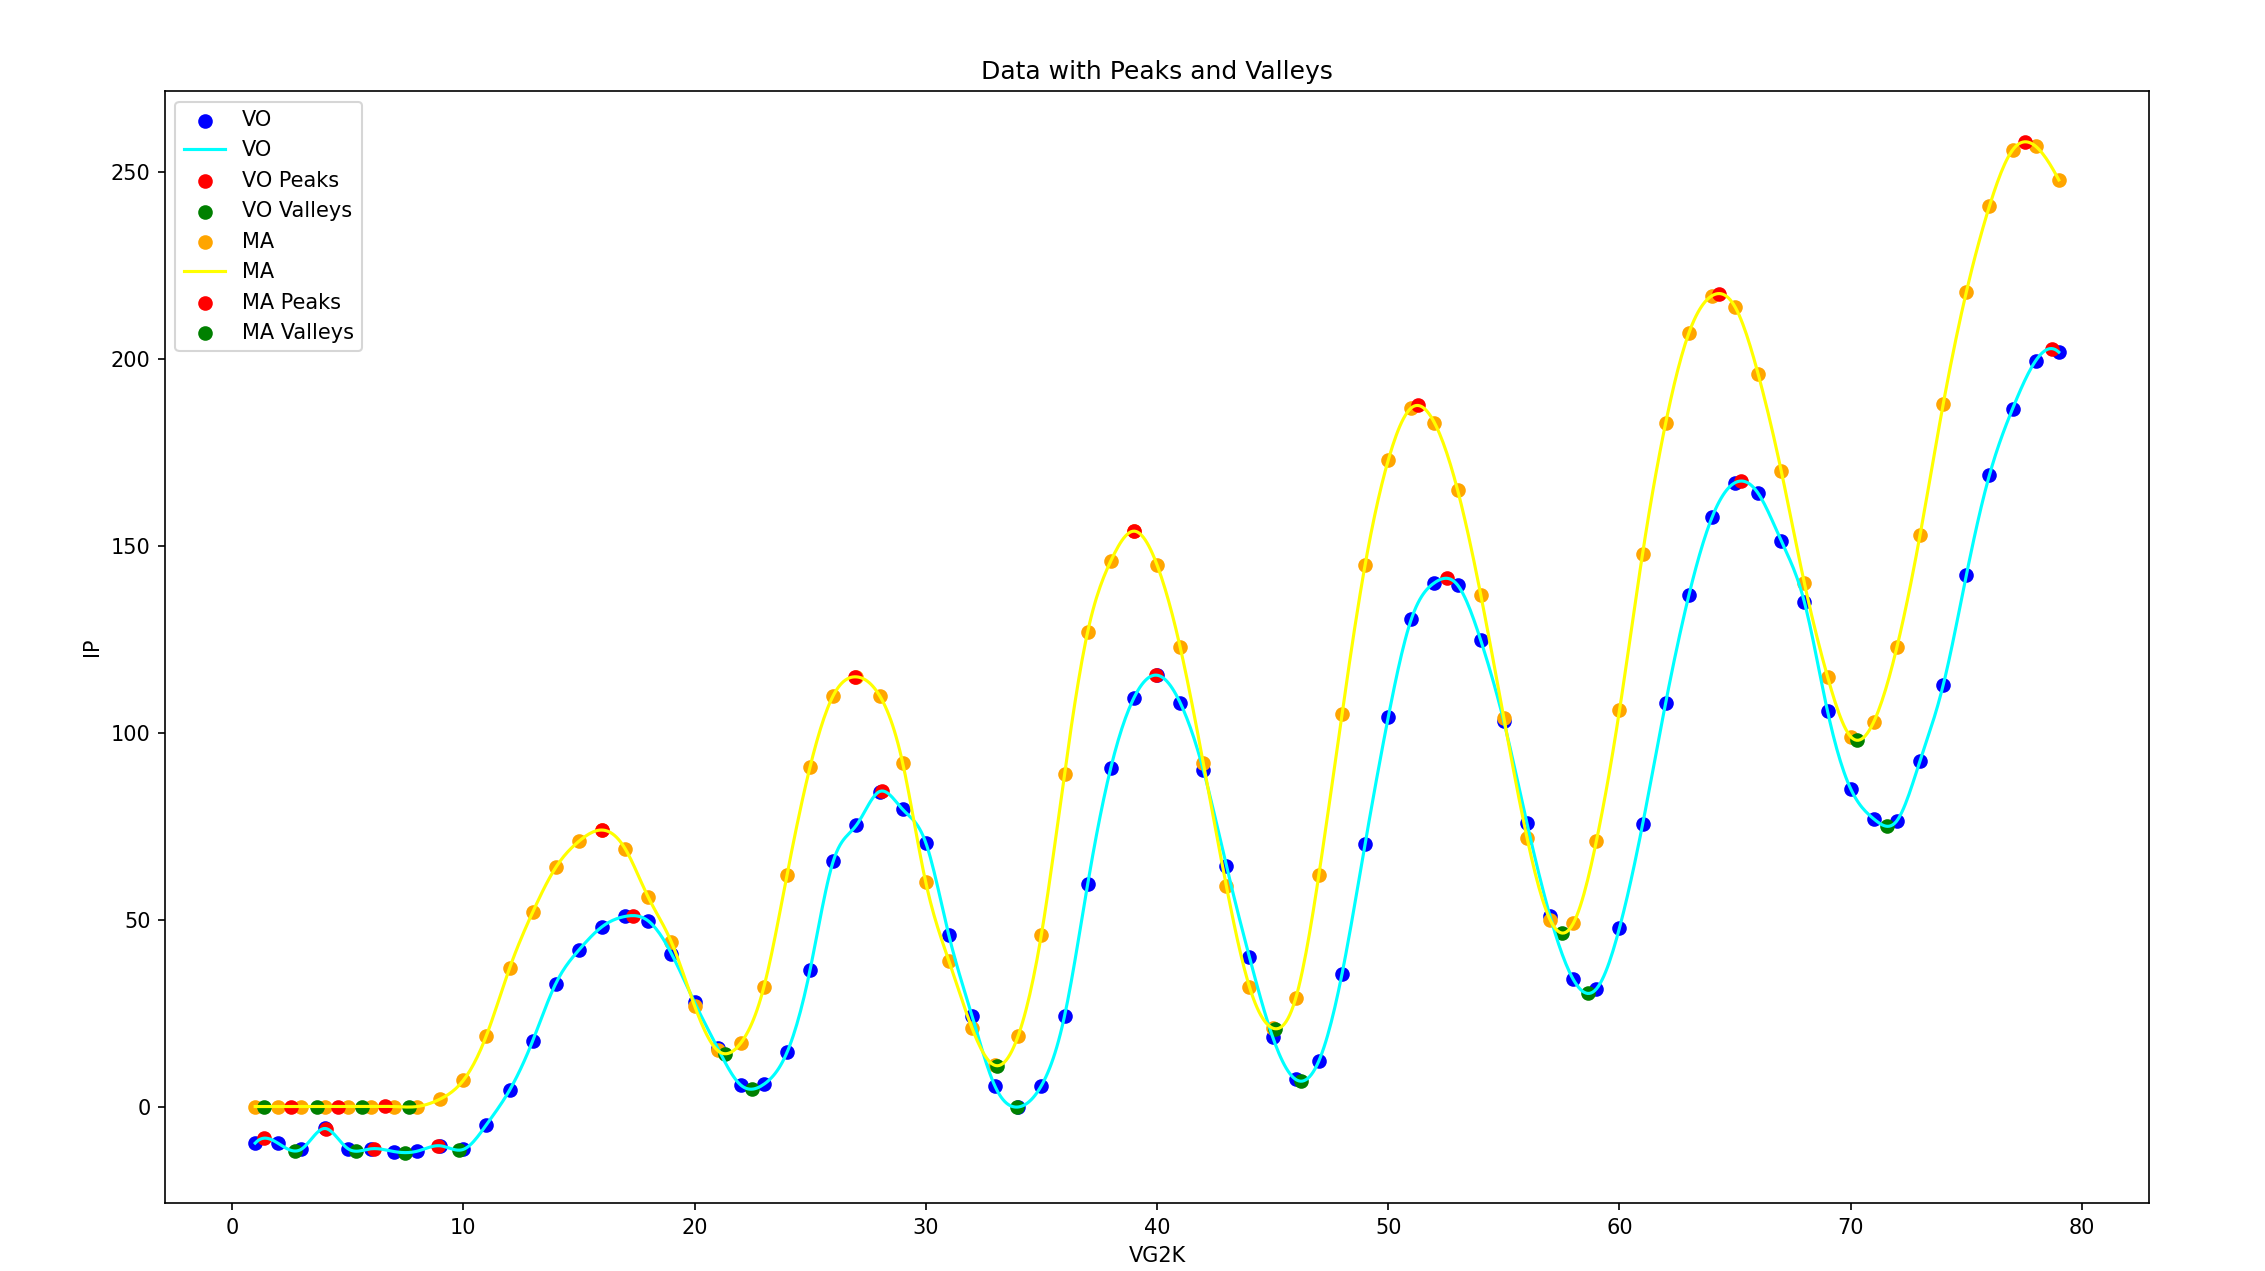
\includegraphics[width=0.8\linewidth]{拟合2.png}
		\caption{曲线寻峰寻谷}
		\label{}
	\end{figure}
提取图像中的峰谷数据,删除电压较小时的错误数据,得出如下实验峰谷结果。
	\begin{table}[H]
		\centering
		\begin{tabular}{ccccc}
		\hline
		& 自动\_peaks & 自动\_valleys & 手动\_peaks & 手动\_valleys\\
		\hline
		1 & 8.885886 & 9.822823 & 15.990991 & 7.636637 \\
		2 & 17.318318 & 22.471471 & 26.921922 & 21.300300 \\
		3 & 28.093093 & 33.948949 & 39.024024 & 33.090090 \\
		4 & 39.960961 & 46.207207 & 51.282282 & 45.114114 \\
		5 & 52.531532 & 58.621622 & 64.321321 & 57.528529 \\
		6 & 65.258258 & 71.582583 & 77.516517 & 70.255255 \\
		\hline
		\end{tabular}
		\caption{拟合图像寻峰寻谷}
		\label{tab:my_table}
		\end{table}
		计算每一组数据之间的峰-峰间距,谷-谷间距,得出如下结果,其中最后一行为各列数据取平均的结果。所有数据的平均值为$\bar{V}_{0}=11.914114\mathrm{V}$
		\begin{table}[H]
			\centering\caption{峰-峰、谷-谷间距}
			\begin{tabular}{cccc}
			\hline
			 自动峰间距 & 自动谷间距 & 手动峰间距 & 手动谷间距 \\
			\hline
		
			 8.432432 & 12.648648 & 10.930931 & 13.663663 \\
			 10.774775 & 11.477478 & 12.102102 & 11.789790 \\
			 11.867868 & 12.258258 & 12.258258 & 12.024024 \\
			12.570571 & 12.414415 & 13.039039 & 12.414415 \\
			12.726726 & 12.960961 & 13.195195 & 12.726726 \\
			\hline
			  11.274874 & 11.952352 & 12.305905 & 12.123324 \\
			  \bottomrule
			\end{tabular}
			
			
		\end{table}
		\subsubsection{两种结果对比分析}
		
		
	\begin{enumerate}
		\item 相同点
		
		\quad \quad 两种方法所得的图像的形态相似,都是电流$I_{P}$随着电压$V_{G_{2K}}$增加而不断地上升、下降,出现一系列峰和谷。并且观察实验最终数据,两种方法的峰谷间距的结果也较为接近,说明从实验结果来看,都较为准确。

		 \item 不同点
		 
		\quad \quad 手动测量的数据都略大于自动测量数据,观察图像中的两条曲线的高度可以发现手动测量数据(MA线)始终大于自动测量数据(VO线),这可能是因为,在此实验中,灯丝的温度稳定是一个非常重要的条件,而由于自动测量的电压上升太快,导致灯丝在每一个电压值上的温度并未稳定,这就导致了灯丝热电子的发射率降低,从而使得自动测量的数据始终低于手动测量的峰值数据。

		\quad \quad 手动测量的曲线呈现一个前置的效果,即峰谷值对应的电压比自动测量曲线小,这可能是因为自动测量的每一电压值的停留时间较短,导致了电流尚未稳定,而手动测量的停留时间较长,所以所得的实验数据更为精确,对于停留时间的影响,具体讨论见3.2.3。
	
         \item 综合讨论
         
		 \quad \quad  两实验方式各有优劣,自动测量胜在测量精度更高、速度更快,可以短时间内获得大量数据;手动测量则是会有足够的时间让电流稳定,实验数据总体上准确,但是由于仪器的限制,导致了实验数据的精度不高。
\end{enumerate}
	%
	\subsubsection{停留时间影响实验结果的讨论}
	3.2.2中对于手动停留时间较长从而影响峰谷值的讨论,为了验证此项猜想,在实验过程中我进一步完成了调整时间间隔为3s的实验,将实验数据导出并与手动测量数据共同绘制实验图像。

	\textbf{观察此图像与图6(较小时间间隔的自动测量),会发现无论是数据之间的高度差距亦或是手动曲线的前置都变小了,这说明对于自动测量来说,可以通过调大时间间隔从而保证在自动记录数据时所得到的数据是在电流稳定的情况下输出的,验证了3.2.2中对于两种不同测量方式数据差异的原因的讨论。}

	若想消除此误差,可以通过增大时间间隔的方式来消除自动测量的弊端,这样既保证了实验数据的精确,也使得实验结果符合实际。
	\begin{figure}[{H}]
		\centering
		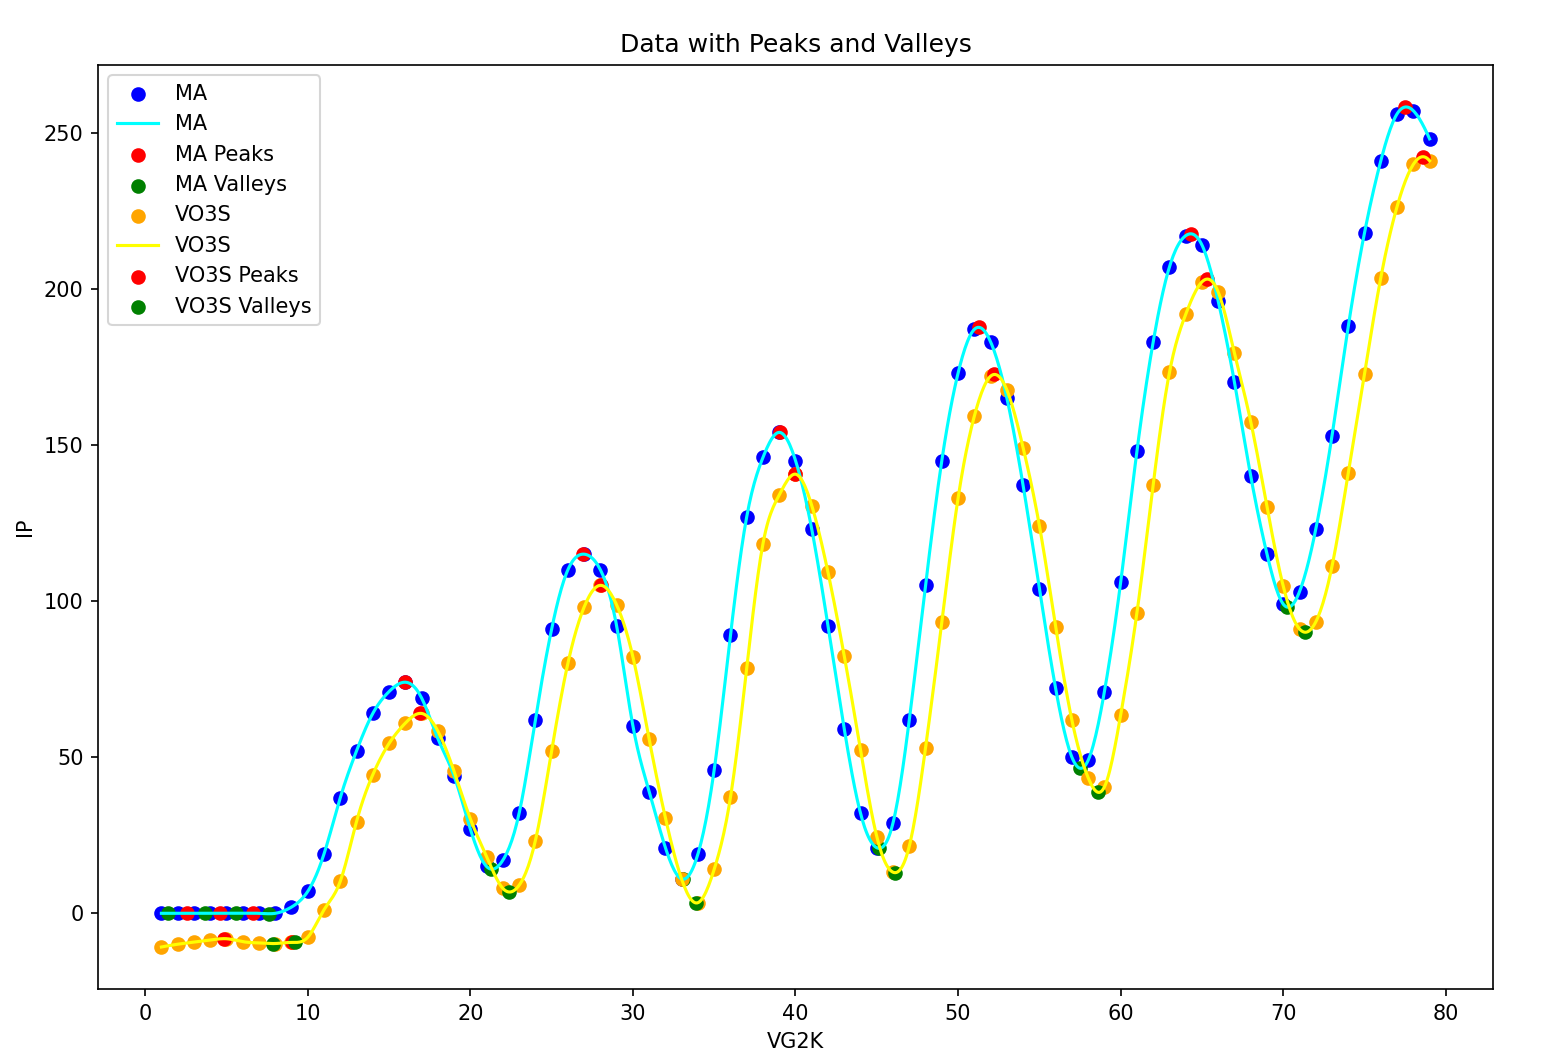
\includegraphics[width=0.8\linewidth]{拟合3.png}
		\caption{增大时间间隔后与手动测量峰谷对比}
		\label{}
	\end{figure}

	\subsection{对于实验结果定性分析}
	\begin{enumerate}
		\item 实验参数定性分析
		
		\quad \quad 实验中存在众多参数,而本实验仅研究了灯丝电压对$I_P{\sim}V_{G_2K}$曲线的影响,下面对于此实验中根据出厂参数设置的参数进行定性分析。

		\quad \quad \textbf{灯丝电压 $V_L$:灯丝电压决定了灯丝的温度,从而影响热电子的发射数量。随着$V_L$的增加,释放的电子数量增加,这导致图中峰值电流($I_{Pmax}$)增大,同时曲线的起伏更加明显,因为更多电子会与加速区域中的气体分子发生碰撞。峰和谷之间的差值也会随着$V_L$的增大而增大。}

		\quad \quad \textbf{收集电压 $V_{G_1K}$:$V_{G_1K}$的作用是收集热发射电子,将它们引入加速区域。如果$V_{G_1K}$增加,在相同的灯丝电压条件下,更多的电子会被收集到加速区。这使得$I_{P}{\sim}V_{G_{2}K}$曲线的起始电压降低。}

		\quad \quad \textbf{拒斥电压 $V_{G_2P}$:抑制电压用于将通过加速区但未到达阳极的电子推回栅极,并使得$V_{G_{2}K}$增大时$I_P$趋向饱和,但是其不可过大,否则会导致电离现象的产生}

		\item 对于波谷点电流定性分析
		
		\quad \quad 观察$I_P{\sim}V_{G_2K}$曲线可以发现谷值处的电流不会降至零,并且随着$V_{G_2K}$的增大而增加。这可以用以下方式解释:

		\quad \quad 由于电子在加速区可能会与原子发生碰撞,但这种碰撞是概率事件,并不一定每个电子都会发生碰撞。因此,总有一些电子能够直接通过加速区而未发生碰撞,直接到达板极,从而形成板极电流。这是为什么即使在曲线的谷值处,电流也不会完全降至零。

		\quad \quad 当加速电压$V_{G_2K}$增大时,这些电子的能量也随之增加。因此,电子以更高的能量通过加速区,直接到达板极的概率增加。这种情况下,即使在碰撞的最小点,电子仍然可能以足够的能量到达板极,导致谷值处的电流上升。

		\quad \quad 总之,谷值电流不为零的原因在于,电子通过加速区时,有一定概率未发生碰撞而直接到达板极。而随着加速电压的增大,电子的能量也增加,这种直接到达板极的电子数量会增加,因此谷值电流会随之增大。

		\item 对于原子对电子的弹性散射的讨论
	
		\quad \quad 正如在实验原理部分,对于电子与氩原子发生弹性碰撞和非弹性碰撞的讨论,在弹性碰撞下,由于原子比电子的质量大得多,所以电子的速度的该变量较小,动能损失也较小,会继续在电场中获得能量。

		\quad \quad 但是由于弹性碰撞会导致电子运动方向的改变,这可能会降低到最终测量电流得到强度,可能会有一部分电子最终飞向器壁。


	\end{enumerate}
	

	

	
	
	%
	\subsection{对于实验结果定量分析}

	\begin{enumerate}
		\item 误差分析
	
		\quad \quad 实验测得最终该数据为$\bar{V}_{0}=12.043794\mathrm{V}.$,$\text{其物理意义为氩原子的第一激发电位}V_0$

		\quad \quad 而氩原子的第一激发电位的标准值为13.08V,$\text{相对误差}\delta=\frac{12.043-13.08}{13.08}\times100\%\approx7.92\%$

		\quad \quad 经过查找资料显示,氩原子基态与第一激发态之间存在两个亚稳态。其中,基态的电势为$U_0=15.76V$, 两个亚稳态的电势分别为$U_1^{\prime}=4.21V$, $U_1^{\prime\prime}=4.04V$,第一激发态的电势为$U_{1}=2.68V$。\small [1]
		
		\quad \quad 基态与两个亚稳态之间的电势差为$\Delta U_{1}^{\prime}=11.55\mathrm{V},\Delta U_{1}^{\prime\prime}=11.72\mathrm{V}。$
		\begin{figure}[H]
			\centering
			\begin{minipage}[b]{0.4\linewidth}
				\centering
				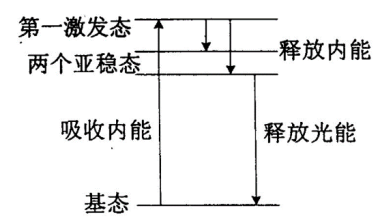
\includegraphics[width=1.0\linewidth]{亚稳态.png}
				\caption{氩原子存在亚稳态示意图}
			\end{minipage}
			\quad % 为了在图和文字之间增加一些间距
			\begin{minipage}[b]{0.5\linewidth}
				\quad \quad 而这两个亚稳态的电势差的数值就很接近实验所测的数值,误差更小,所以可以初步判断实验所测得 $V_0 = 12.043794\mathrm{V}$ 为亚稳态与基态之间的电势差。
				
				\quad \quad \textbf{但是仍存在一定的实验误差,这可能是因为,在实验中采用了Pyhon代码进行拟合运算得出的峰值,并没有进行实际测量到峰值,此外在3.2.2中已经讨论了较短的停留时间的影响,这些都可能会引入实验误差,而可以通过减小测量的步长,增大停留时间来进行多次测量,可能会得到更加精确的数值。}
			\end{minipage}
		\end{figure}
		
		

		\item 建模计算
		
		对于按照出厂参数设置的实验数据进行讨论,绘制图像,并对图像的峰点和谷点进行拟合。
		\begin{figure}[{H}]
			\centering
			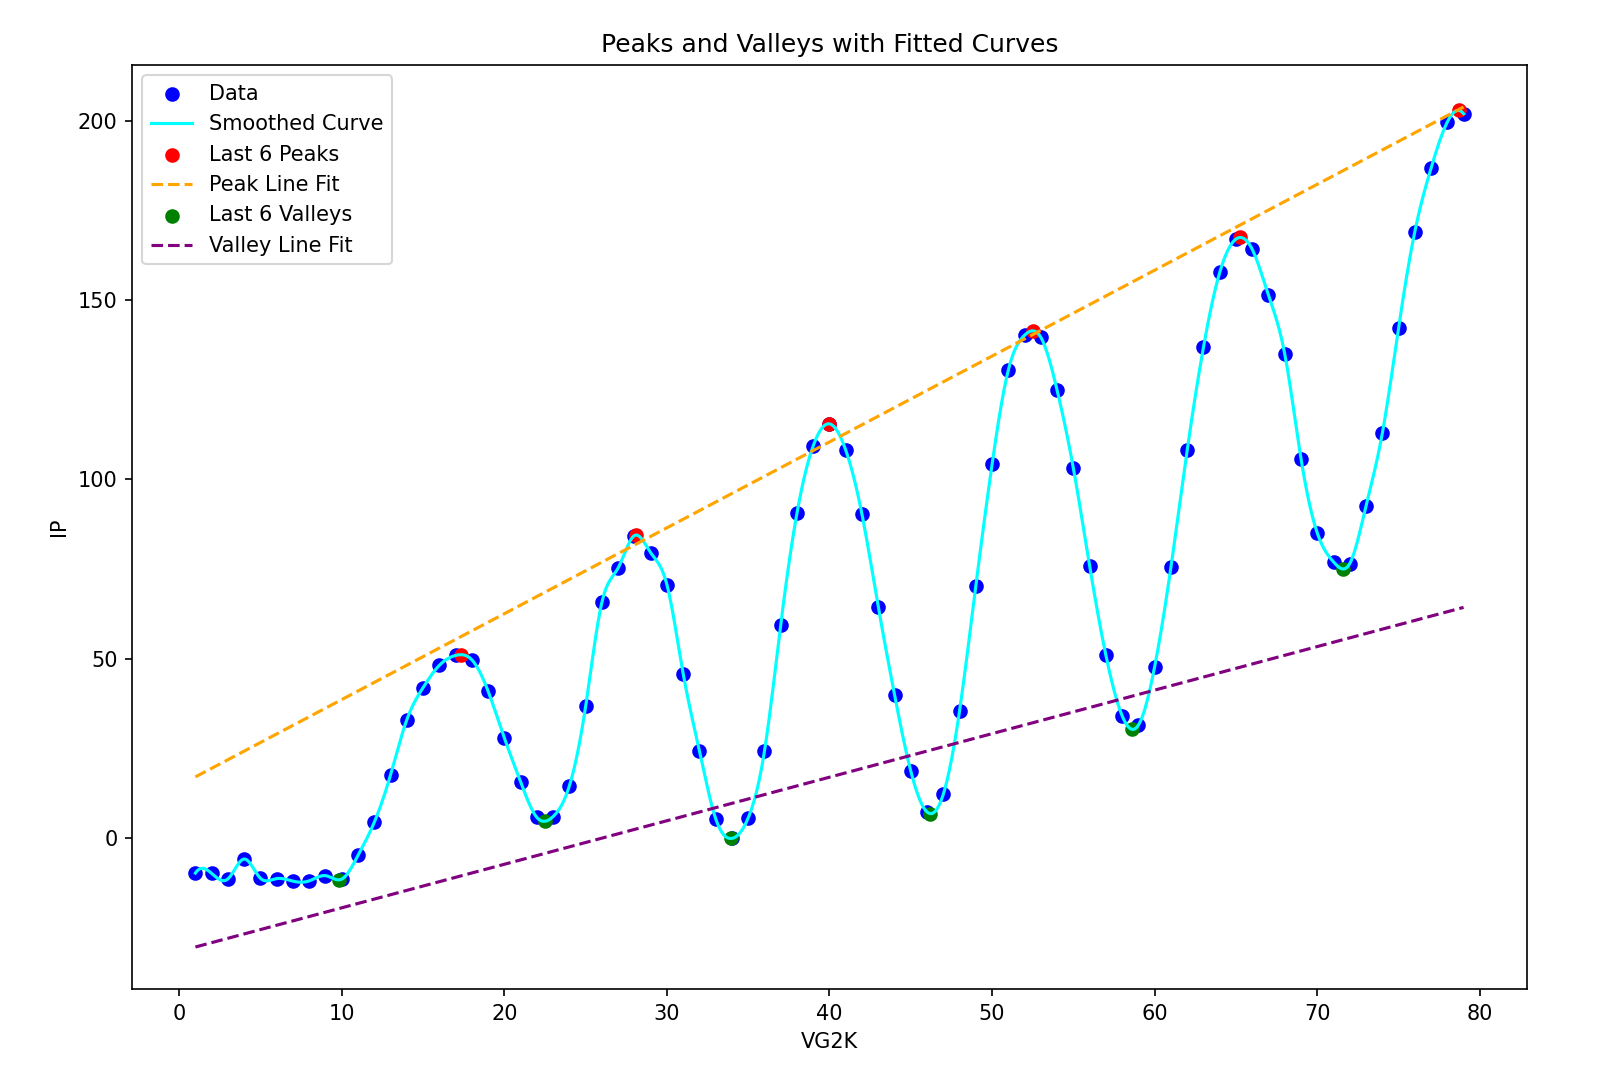
\includegraphics[width=0.45\linewidth]{拟合4.png}
			\caption{直线拟合图像}
			\label{}
		\end{figure}

		其中峰点拟合直线的相关系数$R^2=0.99535$\quad 谷点拟合直线的相关系数仅有$R^2=0.79083$

		这说明电流峰值与电压存在线性关系,现对此进行推导。

		\begin{figure}[{H}]
			\centering
			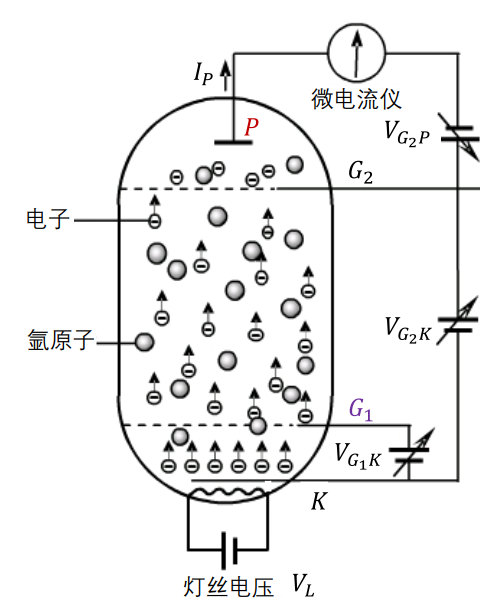
\includegraphics[width=0.4\linewidth]{原理图.png}
			\caption{F-H管}
			\label{}
		\end{figure}
		如图10所示以灯丝中心为原点,建立平面直角坐标系
		电子从灯丝射出,受加速电压加速后到达P。
		$$I=neSv_y$$
		$$v_y=\sqrt{\frac{2eV}m}\propto\sqrt{V}$$
		$n$为电子数密度,$e$为电子的电荷量,S为极板横截面积,$v_y$为电子的纵向速度。

		对于$v_x$,其满足麦克斯韦-玻尔兹曼分布一维形式
		$$f(v_x)=\left(\frac m{2\pi k_BT}\right)^{\frac12}\exp\left(-\frac{mv_x^2}{2k_BT}\right)$$
		
		室温下指数项可忽略,故最终得出$v_x\propto\sqrt{\frac1V}$

        并且$v_x$对于n属于反比关系(速度过快就会飞到器壁上),所以$n\propto\sqrt{V}$
        
		最终得出
		$$I=neSv_y\propto V$$
       而峰点拟合直线的相关系数$R^2=0.99535$,证明模型正确。

	   对于谷点的拟合曲线,尚未有较好的思路判断碰撞氩原子后对于电流的影响,但至少已经确定并不是简单一次直线关系。

	   \item 实验参数定量分析
	   
	   相关理论公式参照建模计算中的模型。

	   对于灯丝电压 $V_L$:电压越高,数密度$n$越高,故电流$I$越高。

	   对于收集电压 $V_{G_1K}$:由于模型计算中所用的电压是指整个腔体内的电压,故根据收集电压的方向可知,其越高则总体电压$V$越高,则电流$I$越高。

	   对于拒斥电压 $V_{G_2P}$:判断其方向可以说明,其越高则总体电压$V$越低,则电流$I$越低

	   只需要将相关数据代入到模型计算中的公式中,便可计算出相关理论数值。
	   
	   当然由于此模型存在很多理想化假设,还需要更多的实验数据进行完善和优化。



	   
	   \item 激发态退回基态的计算
	   
	   由$E=\frac{hc}\lambda$可知,对于第一激发态的电子,返回基态时发射的光子波长
$$\lambda=\frac{hc}{E}=\frac{3\times10^8\times6.626\times10^{-34}}{13.08\times1.6\times10^{-19}}\approx94.98\mathrm{nm}$$
基本上小于金属的极限波长,故这些光子可以产生光电效应。

通过此项计算也可以使用光谱仪对氩原子的第一激发态的发光光谱进行测量,光谱仪的频段保证涵盖计算所得结果即可。

而汞原子的第一激发电位为$4.9V$,故可以计算得出,返回基态时波长约为$253nm$,选取涵盖此频段的光谱仪即可。
		
	\end{enumerate}
	\subsection{实验结论}
	\textbf{$I_P{\sim}V_{G_2K}$曲线所展示的峰谷图像显示出原子至吸收特定能量的电子,从而确定原子的定态能级。}
	

	\textbf{实验的结果与理论值存在一定误差,这可能是由于氩原子亚稳态的存在,此外仪器与测量方式可能引入一定的误差。}

	\textbf{对于手动和自动两种测量方式,手动时间更长,精度较低,但是总体数据更准确,自动效率高,精度较高,但是可能存在较大误差,通过进一步分析,可以增大停留时间来减小自动测量的误差。}

	\textbf{通过对于实验的建模和实验结果的拟合,进行定量分析,总结出峰值电流的线性关系。}
	% 结语部分
	\clearpage
	
	% 小标题
	\section{CA2 夫兰克-赫兹实验:原子定态能级的观测  \quad\heiti 结语}
	% ---
	
	% 总结、杂谈与致谢
	\subsection{实验心得和体会、意见建议等}
	\begin{enumerate}
		\item 实验过程较为简单,实验仪器的完善度比较成熟,可以更加系统的对于实验结果进行分析。
		\item 可以运用相关知识进行推导,实验总体的理解程度较深。\item \textbf{本实验报告采用LATEX编辑,实验所有要求内容均包含于本实验报告中}
	\end{enumerate}
	\quad \large \textbf{感谢您对于此篇实验报告的阅读与批改,祝您工作顺利!}
	

	% 附件
	\subsection{附件}
	参考文献

	[1]朱筱玮.氩原子的第一激发电位[J].西北大学学报:自然科学网络版,2006,4(6):0245[2006-11-10].

	\begin{figure}[H]
		\begin{minipage}[b]{0.3\linewidth}
		  \centering
		  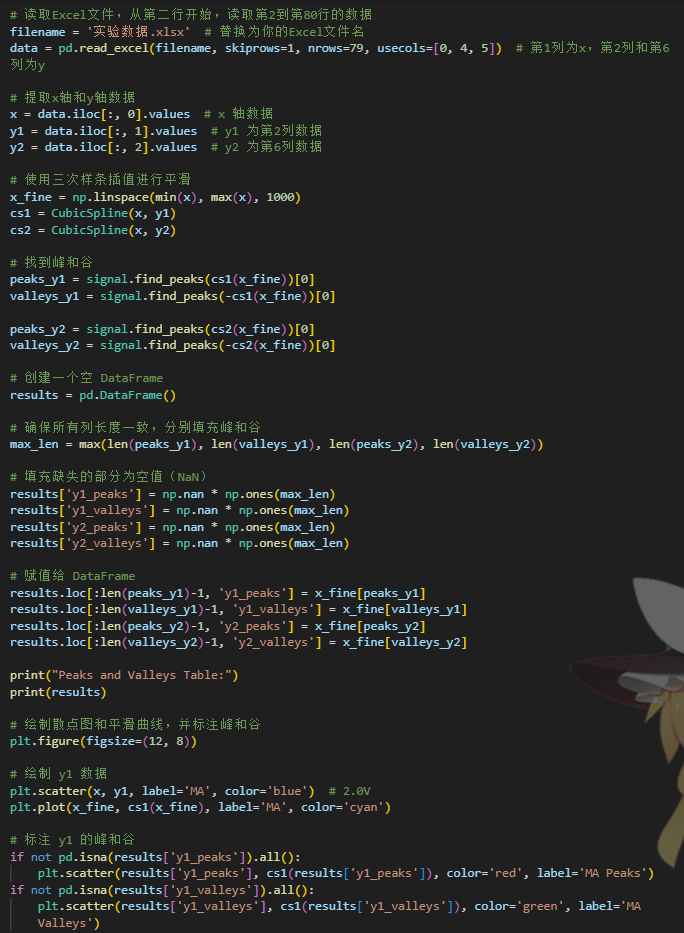
\includegraphics[width=\linewidth]{代码.png}
		  \caption{拟合参考代码}
		\end{minipage}
		\hfill
		\begin{minipage}[b]{0.3\linewidth}
		  \centering
		  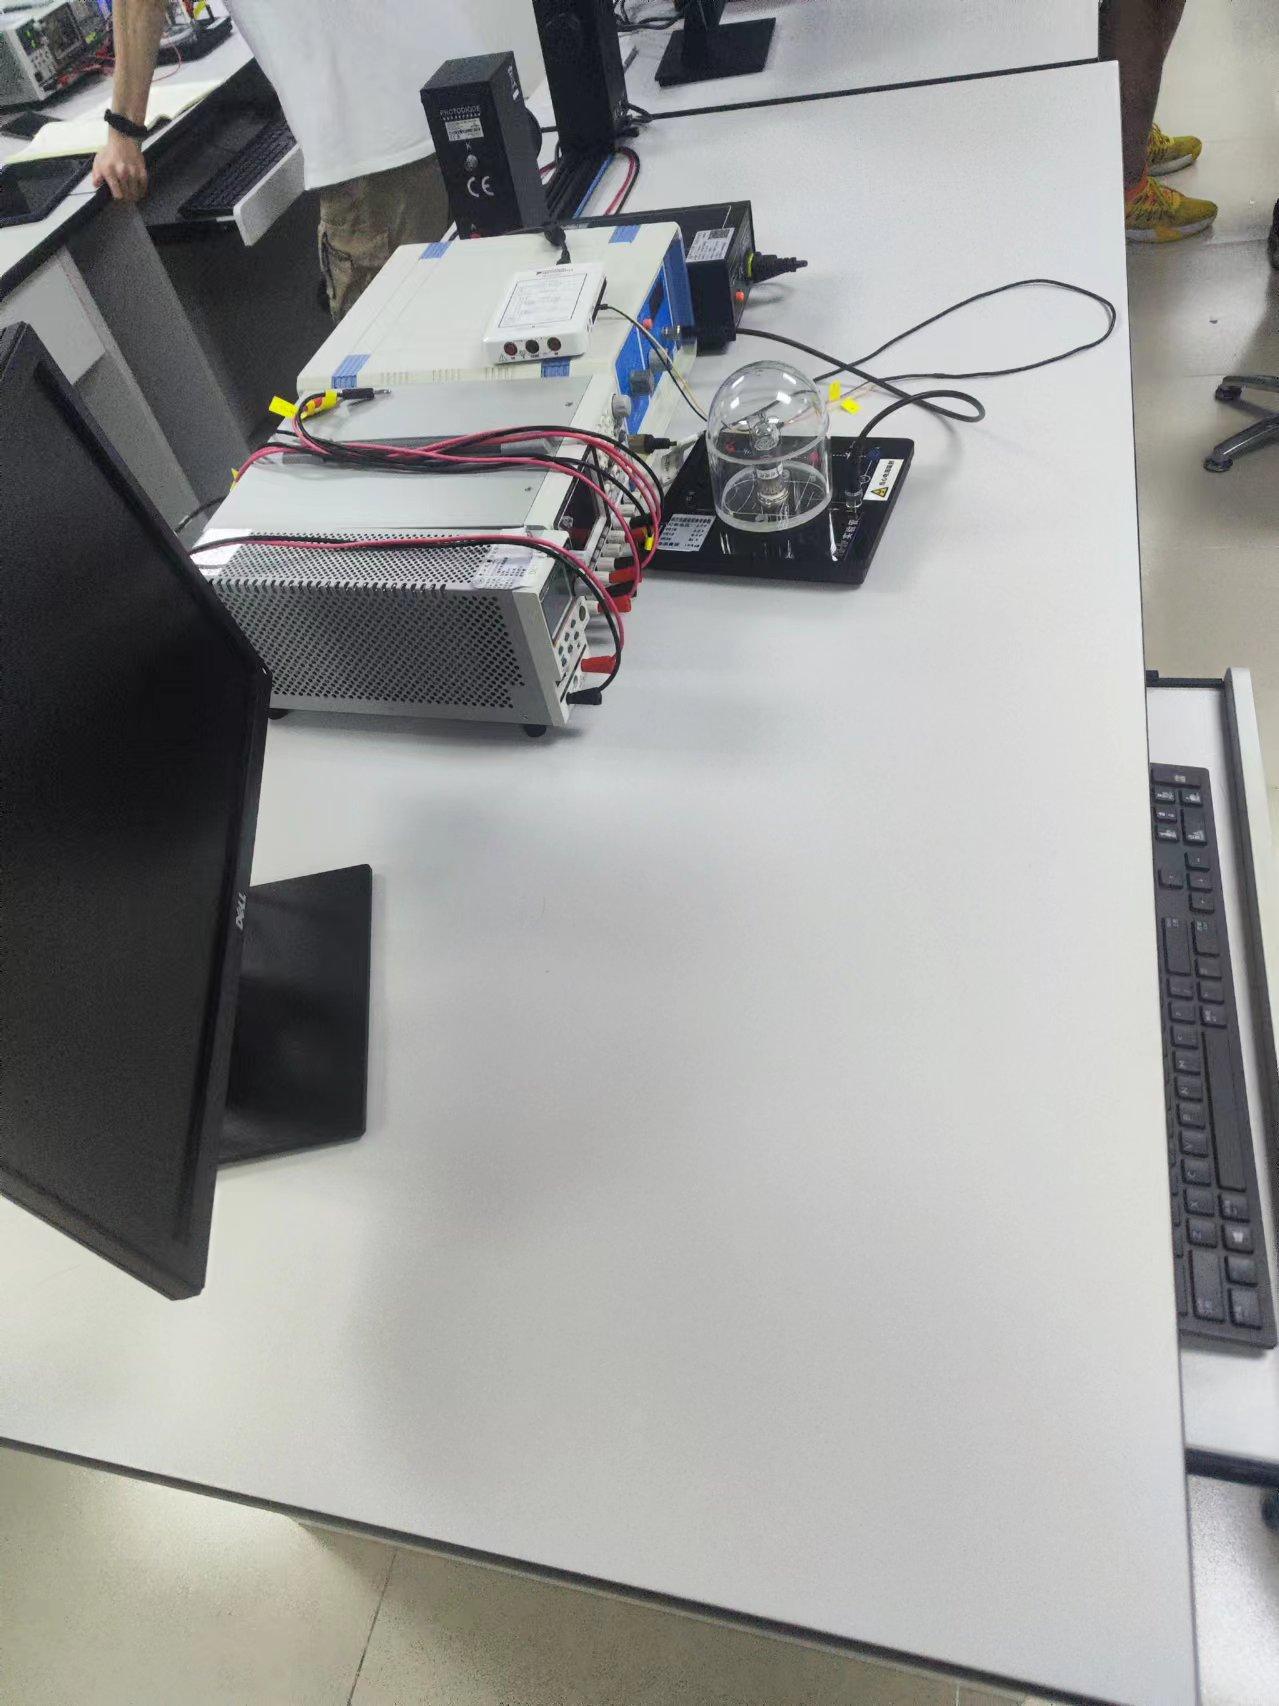
\includegraphics[width=\linewidth]{桌面.jpg}
		  \caption{整理桌面}
		\end{minipage}
		\hfill
		\begin{minipage}[b]{0.3\linewidth}
		  \centering
		  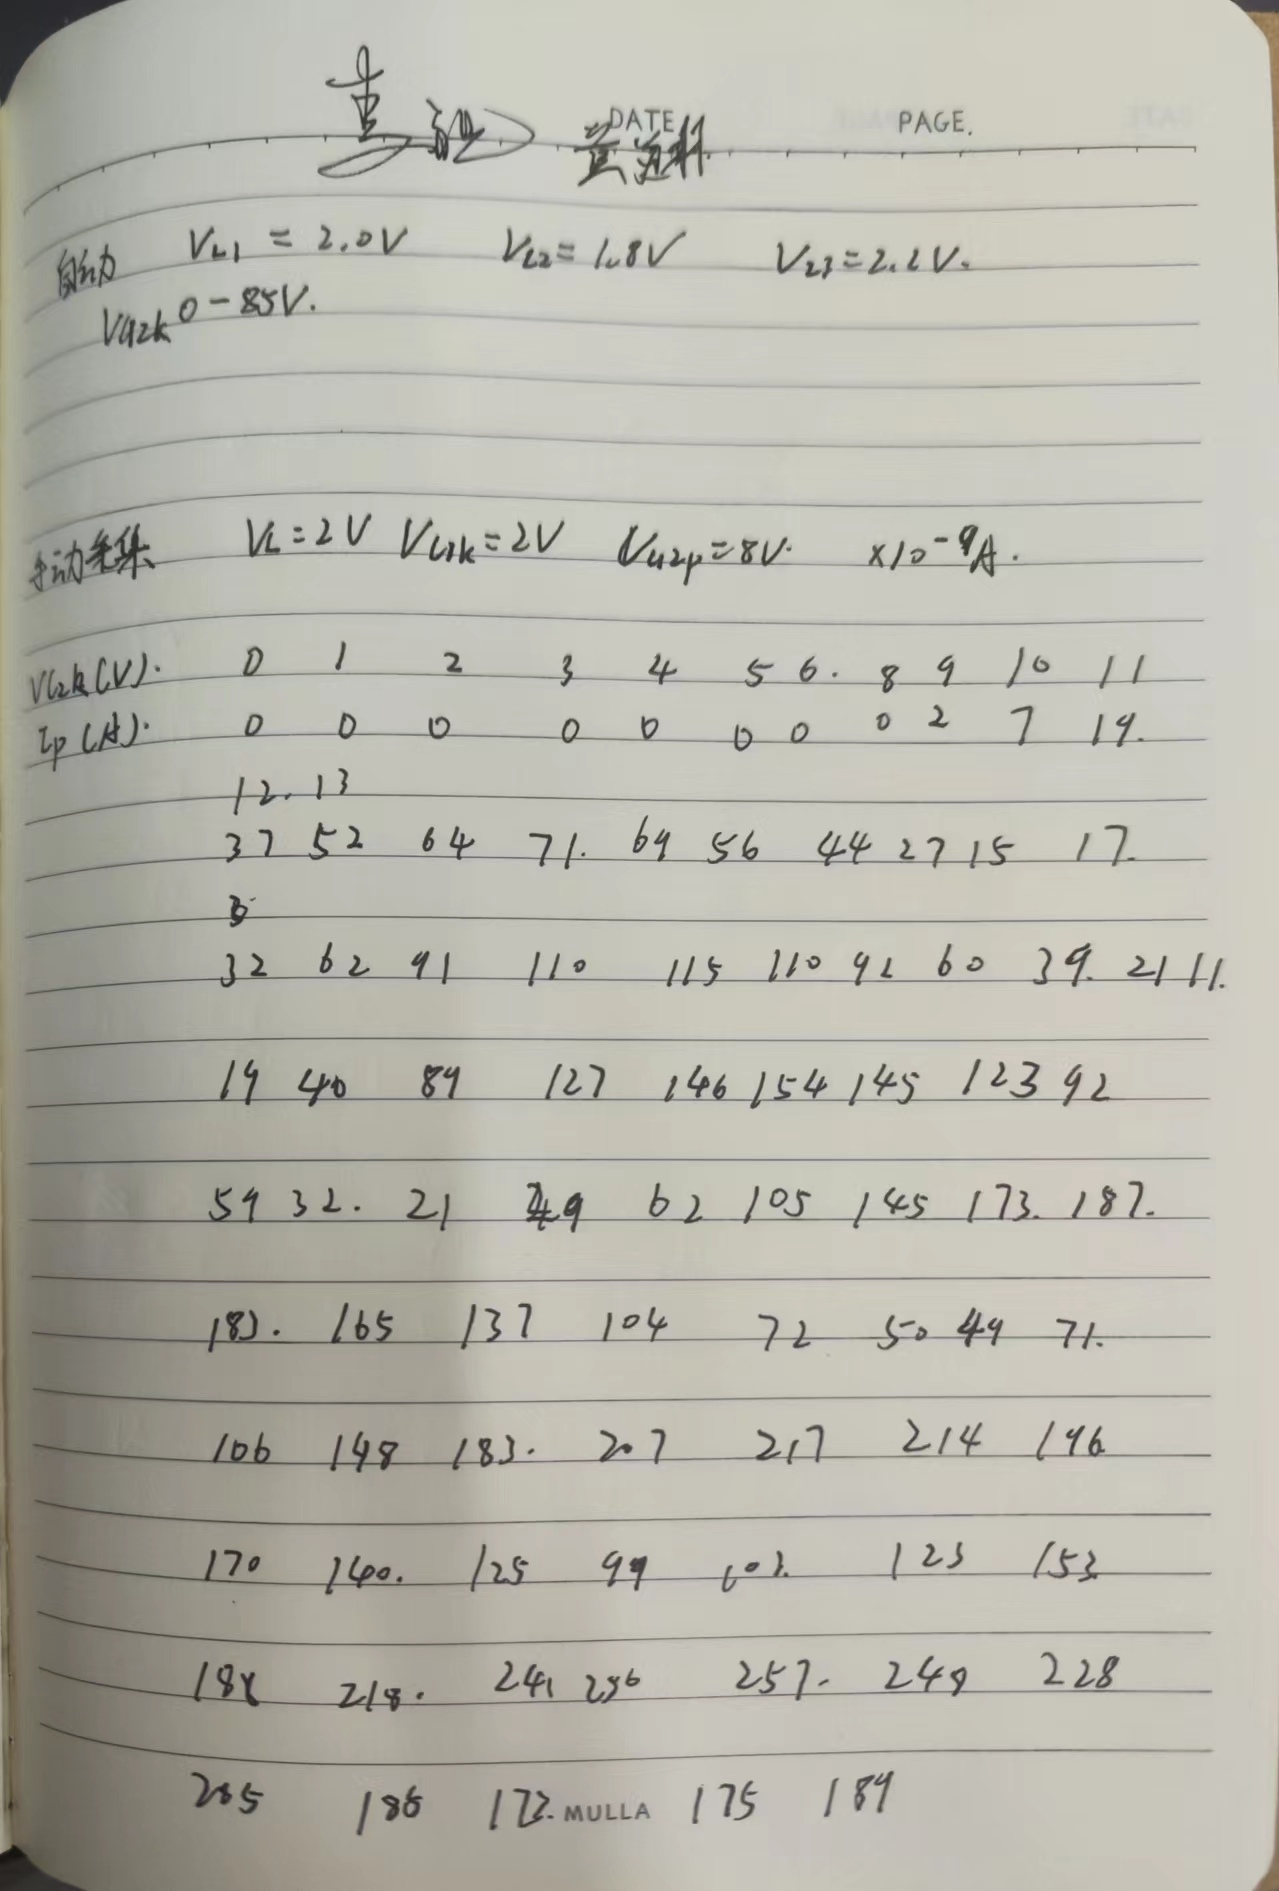
\includegraphics[width=\linewidth]{原始数据.jpg}
		  \caption{实验原始数据}
		\end{minipage}
	\end{figure}
	
	
\end{document}